\documentclass[11pt,a4paper]{article}

\usepackage[
  inner=25mm,
  outer=21mm,
  top=24mm,
  bottom=26mm,
  headsep=7mm,
  footskip=12mm,
  includeheadfoot
]{geometry}
\usepackage{fontspec}
\usepackage{polyglossia}
\setmainlanguage{russian}
\setotherlanguage{english}
\setmainfont{CMU Serif}[Ligatures=TeX]
\setsansfont{CMU Sans Serif}[Ligatures=TeX]
\setmonofont{CMU Typewriter Text}[Scale=0.92]
\usepackage{amsmath,mathtools,bm}
\usepackage{unicode-math}
\setmathfont{Latin Modern Math}
\usepackage{booktabs,longtable,array,ragged2e,multirow}
\usepackage{graphicx}
\usepackage{caption}
\usepackage{subcaption}
\usepackage{xcolor}
\usepackage{hyperref}
\usepackage{xurl}
\usepackage{tocloft}
\usepackage{enumitem}
\usepackage{fancyhdr}
\usepackage{microtype}
\usepackage{listings}
\usepackage{indentfirst}
\usepackage{titlesec}
\usepackage{placeins}

\graphicspath{{docs/figures/}{figures/}{docs/}{./}}
\hypersetup{
  pdftitle={Подробное руководство MBS-fast},
  pdfauthor={MBS-fast},
  colorlinks=true,
  linkcolor=blue!38!black,
  urlcolor=blue!45!black,
  citecolor=blue!38!black,
  bookmarksopen=true,
  bookmarksnumbered=true
}

\pagestyle{fancy}
\fancyhf{}
\lhead{MBS-fast}
\rhead{Руководство пользователя и разработчика}
\cfoot{\thepage}
\setlength{\headheight}{15pt}
\setlength{\parindent}{1.55em}
\setlength{\parskip}{0pt}
\linespread{1.08}
\emergencystretch=2em
\raggedbottom

\titleformat{\part}[display]
  {\centering\normalfont\Large\bfseries}
  {Часть~\thepart}{0.5em}{\LARGE}
\titlespacing*{\part}{0pt}{1.2em}{0.2em}
\titleformat{\section}
  {\normalfont\Large\bfseries}{\thesection.}{0.65em}{}
\titleformat{\subsection}
  {\normalfont\large\bfseries}{\thesubsection.}{0.6em}{}
\titleformat{\subsubsection}
  {\normalfont\normalsize\bfseries}{\thesubsubsection.}{0.55em}{}
\titlespacing*{\section}{0pt}{2.3em plus 0.5em minus 0.3em}{0.8em}
\titlespacing*{\subsection}{0pt}{1.7em plus 0.4em minus 0.2em}{0.55em}
\titlespacing*{\subsubsection}{0pt}{1.3em plus 0.3em minus 0.2em}{0.4em}
\setcounter{tocdepth}{1}
\setcounter{secnumdepth}{3}
\setlist{leftmargin=1.7em,itemsep=0.25em,topsep=0.45em,parsep=0pt}
\setlength{\textfloatsep}{14pt plus 3pt minus 2pt}
\setlength{\intextsep}{12pt plus 3pt minus 2pt}
\setlength{\abovedisplayskip}{8pt plus 2pt minus 2pt}
\setlength{\belowdisplayskip}{8pt plus 2pt minus 2pt}

\newcolumntype{L}[1]{>{\RaggedRight\arraybackslash}p{#1}}
\newcolumntype{C}[1]{>{\Centering\arraybackslash}p{#1}}
\newcommand{\code}[1]{\texttt{\small\detokenize{#1}}}
\newcommand{\flag}[1]{{\small\nolinkurl{#1}}}
\newcommand{\vect}[1]{\symbf{#1}}
\newcommand{\matr}[1]{\symbf{#1}}
\newcommand{\dd}{\,\mathrm{d}}
\newcommand{\ii}{\mathrm{i}}
\newcommand{\Real}{\operatorname{Re}}
\newcommand{\Imag}{\operatorname{Im}}
\newcommand{\conj}[1]{\overline{#1}}
\newcommand{\norm}[1]{\left\lVert #1 \right\rVert}
\newcommand{\SectionNote}[1]{%
  \par\medskip
  \noindent\fcolorbox{blue!30!black}{blue!4}{%
    \parbox{\dimexpr\linewidth-2\fboxsep-2\fboxrule\relax}{\small #1}}%
  \par\medskip
}

\lstdefinestyle{cmd}{
  basicstyle=\ttfamily\footnotesize,
  breaklines=true,
  columns=fullflexible,
  frame=leftline,
  framerule=0.8pt,
  rulecolor=\color{black!35},
  backgroundcolor=\color{black!2},
  xleftmargin=1em,
  framexleftmargin=0.6em,
  aboveskip=0.8em,
  belowskip=0.8em,
  showstringspaces=false,
  keepspaces=true
}
\lstset{style=cmd}
\setlength{\cftsecnumwidth}{2.8em}
\setlength{\cftsubsecnumwidth}{4.2em}

\begin{document}
\begin{titlepage}
  \thispagestyle{empty}
  \centering
  \vspace*{0.16\textheight}
  {\Huge\bfseries MBS-fast\par}
  \vspace{1.2em}
  {\LARGE Руководство пользователя и разработчика\par}
  \vspace{0.8em}
  {\large Геометрическая и физическая оптика для многогранных частиц\par}
  \vfill
  \begin{minipage}{0.76\textwidth}
    \small
    Документ описывает физическую модель, численные алгоритмы, сборку,
    параметры запуска, форматы данных, ускорение на CPU и GPU, а также
    обязательные проверки точности. В командах используются канонические имена
    параметров из текущего интерфейса программы; устаревшие сокращения указаны
    отдельно и нужны только для воспроизводимости старых сценариев.
  \end{minipage}
  \vfill
  {Редакция от 12 августа 2026 г.\par}
  \vspace{0.5em}
  {Документ для актуального интерфейса командной строки\par}
\end{titlepage}

\pagenumbering{roman}
\section*{О руководстве}
\addcontentsline{toc}{section}{О руководстве}

MBS-fast предназначен для расчёта дальнего рассеяния света многогранными
частицами. Геометрическая стадия строит и трассирует полигональные пучки,
перенося комплексную матрицу Джонса через отражения и преломления. В режиме
физической оптики (PO) каждый выходной пучок дополняется дифракционным интегралом
по его апертуре. После когерентного суммирования амплитуд результат переводится
в матрицу Мюллера и, при необходимости, усредняется по ориентациям частицы.

Руководство рассчитано на два способа чтения. Для первого запуска достаточно
разделов «Быстрый старт», «Сборка и исполняемые файлы», «Параметры командной
строки» и «Обязательные проверки результата». Разделы о трассировке,
коэффициентах Френеля,
дифракционном интеграле и реализации на CPU/GPU предназначены для проверки
физики и модификации кода. Приложения содержат формулы метрик и контрольный
список для воспроизводимого расчёта.

\tableofcontents
\clearpage
\pagenumbering{arabic}

\part{Практическая работа}

\section{Быстрый старт}

\subsection{Сборка проверочного бинарного файла}

Для воспроизводимой проверки сначала собирают CPU-версию и запускают матрицу
коротких тестов интерфейса:

\begin{lstlisting}[language=bash]
make -C cpu -j
make test_release
cpu/bin/mbs_po_mpi --version
\end{lstlisting}

GPU-версия двойной точности собирается отдельной целью. Именно её следует
использовать для проверки точек $0^\circ$ и $180^\circ$ и для сравнения с CPU:

\begin{lstlisting}[language=bash]
make -C gpu fp64 -j
gpu/bin/mbs_po_gpu_double --version
\end{lstlisting}

\subsection{Первый расчёт}

Следующая команда считает гексагональный столбик длиной 100~мкм и диаметром
70~мкм при $\lambda=0.532$~мкм. Сетка ориентаций и углов рассеяния строится из
дифракционной оценки; широтная сетка уменьшает избыточное число азимутальных
узлов около полюсов.

\begin{lstlisting}[language=bash]
CUDA_VISIBLE_DEVICES=0 \
gpu/bin/mbs_po_gpu_double \
  --method po \
  --particle 1 100 70 \
  --refractive-index 1.3116 0 \
  --wavelength-um 0.532 \
  --max-reflections 8 \
  --diffraction-sampling 2 \
  --latitude-phi-grid \
  --backend cuda --threads 16 \
  --cutoff-profile off \
  --output results/column_L100 --close
\end{lstlisting}

Это контрольная, а не самая быстрая конфигурация. Профили отсечения, FFT и
многопроцессорное распределение включают только после сравнения с таким прямым
расчётом на нескольких характерных размерах.

\subsection{Что проверить после завершения}

Расчёт можно использовать дальше, только если одновременно выполнены следующие
условия:

\begin{enumerate}
  \item процесс завершился с нулевым кодом, а выходной файл содержит все строки
    по $\theta$ от $0^\circ$ до $180^\circ$;
  \item в логе нет сообщения о достижении ограничения числа пучков или верхней
    границы адаптивного поиска;
  \item отчёт интегральных величин не содержит статуса
    \code{check_csca_integration};
  \item более мелкая сетка по ориентациям и углам меняет требуемые элементы
    матрицы Мюллера меньше заданной погрешности;
  \item для новой формы хотя бы одна небольшая задача совпадает между CPU и GPU
    двойной точности.
\end{enumerate}

\SectionNote{Завершившийся процесс ещё не означает сошедшийся физический
результат. Глубина трассировки, угловая сетка, ориентационное усреднение,
отсечения слабых пучков и численная точность проверяются независимо.}

\part{Физическая модель и геометрия}

\section{Назначение программы}

MBS-fast решает задачу дальнего рассеяния на частице с плоскими гранями.
В отличие от метода дискретных диполей программа не заполняет объём частицы
расчётными узлами. Она строит геометрические пучки, возникающие после отражений
и преломлений на гранях. Каждый пучок хранит полигон апертуры, направление
распространения, оптический путь и комплексную матрицу Джонса. После
трассировки для каждого выходного пучка вычисляется дифракционный интеграл
физической оптики. Амплитуды суммируются когерентно и преобразуются в матрицу
Мюллера.

\begin{figure}[htbp]
  \centering
  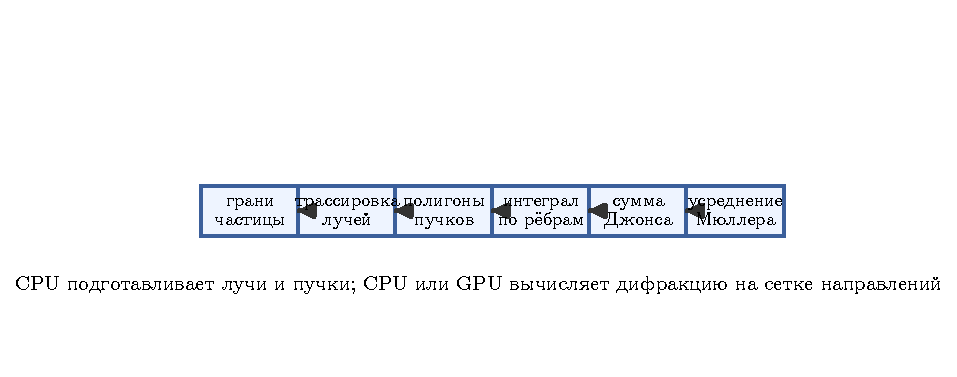
\includegraphics[width=0.96\linewidth]{manual_pipeline_ru.pdf}
  \caption{Последовательность расчёта: геометрия частицы, трассировка,
  коэффициенты Френеля и матрицы Джонса, дифракция, когерентная сумма,
  матрица Мюллера и усреднение по ориентациям.}
\end{figure}

\subsection{Физические уровни модели}

В расчете используются четыре уровня приближения.

\begin{longtable}{L{0.20\linewidth} L{0.31\linewidth} L{0.39\linewidth}}
\caption{Физические уровни модели MBS-fast.}\\
\toprule
Уровень & Что считается & Где появляется в коде \\
\midrule
\endfirsthead
\toprule
Уровень & Что считается & Где появляется в коде \\
\midrule
\endhead
Геометрическая оптика & Пучки отражаются и преломляются на плоских гранях по законам Снеллиуса; малозначимые ветви могут быть отсечены заданным критерием. & \code{src/scattering}, \code{Splitting.cpp}. \\
Френель и Джонс & Поляризационная амплитуда каждой ветви хранится как комплексная матрица Джонса. & \code{Beam::J}, \code{Splitting.cpp}. \\
Физическая оптика & Выходной пучок создаёт дальнее поле, вычисляемое интегралом по его полигональной апертуре. & \code{HandlerPO::ApplyDiffraction*}, ядра CUDA. \\
Ориентационное усреднение & Для ансамбля случайно ориентированных частиц вычисляется взвешенная сумма матриц Мюллера по квадратурной или квазислучайной сетке. & \code{HandlerPOTotal}, \code{TracerPOTotal}. \\
\bottomrule
\end{longtable}

\SectionNote{В режиме PO пучки одной ориентации по умолчанию суммируются
когерентно на уровне амплитуд Джонса. Только после этой суммы строится матрица
Мюллера. Параметр \code{--incoherent} меняет физическую постановку: матрицы
Мюллера отдельных пучков складываются без интерференционных членов.}

\subsection{Обозначения}

\begin{longtable}{L{0.14\linewidth} L{0.76\linewidth}}
\caption{Базовые обозначения, используемые дальше.}\\
\toprule
Символ & Смысл \\
\midrule
\endfirsthead
\toprule
Символ & Смысл \\
\midrule
\endhead
$\lambda$ & Длина волны в микрометрах, задаётся параметром \code{--wavelength-um}. \\
$k=2\pi/\lambda$ & Волновое число во внешней среде. \\
$m=n+\ii\kappa$ & Комплексный показатель преломления частицы относительно внешней среды, задаётся параметром \code{--refractive-index Re Im}. \\
$\vect d$ & Направление распространения текущего луча или пучка. \\
$\vect n$ & Внешняя нормаль грани. В коде знак выбирается так, чтобы ветвление было устойчивым для текущей стороны грани. \\
$\theta,\phi$ & Углы направления наблюдения в дальней зоне. \\
$\vect s(\theta,\phi)$ & Единичный вектор направления наблюдения. \\
$\matr J$ & Комплексная матрица Джонса $2\times2$. \\
$\matr M$ & Вещественная матрица Мюллера $4\times4$. \\
$A$ & Площадь или полигон апертуры; смысл уточняется в конкретной формуле. \\
$N_b$ & Число выходных пучков для одной ориентации. \\
$N_{\mathrm{ori}}$ & Число ориентаций в усреднении. \\
\bottomrule
\end{longtable}

\section{Координатные системы}

\subsection{Лабораторная система}

Лабораторная система фиксирована относительно падающего света. Обычно падающий луч направлен вдоль одной из осей, а частица поворачивается матрицей Эйлера. Для любого вектора $\vect x$ в лабораторной системе используются скалярное произведение $\vect a\cdot\vect b$ и векторное произведение $\vect a\times\vect b$. Все направления лучей нормируются:
\[
  \norm{\vect d}=1,\qquad \norm{\vect s}=1,\qquad \norm{\vect n}=1.
\]

\subsection{Система частицы и повороты Эйлера}

Пусть $\vect x_p$ --- координаты вершины в системе частицы, а $\vect x_l$ --- координаты в лабораторной системе. Поворот задается матрицей
\[
  \vect x_l = \matr R(\alpha,\beta,\gamma)\,\vect x_p.
\]
Полная ориентация твёрдого тела задаётся тремя углами Эйлера или единичным
кватернионом. В основной двухугловой квадратуре MBS-fast явно перебираются
$\beta$ и $\gamma$, а усреднение по лабораторному углу $\alpha$ представлено
азимутальной сеткой направления рассеяния. Поэтому уменьшение числа
азимутальных точек меняет не только вывод кривой, но и точность этого
эквивалентного усреднения. Режим \code{--so3-quaternion} использует это
тождество явно: квазислучайно выбирает только $\beta,\gamma$ в фундаментальной
области симметрии частицы, а интеграл по $\alpha$ вычисляет по азимуту
рассеяния. Для независимой прямой проверки полной группы оставлен режим
\code{--so3-full-quaternion}.

Удобная запись через элементарные повороты:
\[
  \matr R(\alpha,\beta,\gamma)
  = \matr R_z(\alpha)\,\matr R_y(\beta)\,\matr R_z(\gamma).
\]
Здесь
\[
\matr R_z(\chi)=
\begin{pmatrix}
\cos\chi&-\sin\chi&0\\
\sin\chi& \cos\chi&0\\
0&0&1
\end{pmatrix},\qquad
\matr R_y(\chi)=
\begin{pmatrix}
\cos\chi&0&\sin\chi\\
0&1&0\\
-\sin\chi&0&\cos\chi
\end{pmatrix}.
\]

\begin{longtable}{L{0.17\linewidth} L{0.73\linewidth}}
\caption{Смысл углов Эйлера.}\\
\toprule
Символ & Смысл \\
\midrule
\endfirsthead
\toprule
Символ & Смысл \\
\midrule
\endhead
$\alpha$ & Поворот вокруг лабораторной оси падающего луча или начальный азимут, если используется полная SO(3)-сетка. \\
$\beta$ & Наклон оси частицы относительно падающего луча; мера содержит якобиан $\sin\beta$. \\
$\gamma$ & Поворот частицы вокруг собственной оси после наклона. При $\beta=0$ и $\beta=\pi$ все значения $\gamma$ геометрически эквивалентны. \\
\bottomrule
\end{longtable}

\subsection{Система грани и апертуры}

Для каждого выходного пучка строится локальная система апертуры. Нормаль апертуры $\vect n_b$ берется из последней грани или из нормали пучка, а две оси в плоскости обозначим $\vect h_b$ и $\vect v_b$:
\[
  \vect h_b\cdot\vect n_b=0,\qquad
  \vect v_b\cdot\vect n_b=0,\qquad
  \vect h_b\cdot\vect v_b=0.
\]
Точка $\vect r$ в лабораторной системе проектируется в координаты апертуры:
\[
  x = (\vect r-\vect r_c)\cdot\vect h_b,\qquad
  y = (\vect r-\vect r_c)\cdot\vect v_b,
\]
где $\vect r_c$ --- центр полигона пучка. Именно эти $x,y$ попадают в \code{BeamEdgeData}: массивы вершин, наклоны ребер и признаки валидности ребер.

\subsection{Система рассеяния}

Для направления наблюдения $\vect s$ строятся две поперечные оси. В коде используется опорный вектор \code{vf} и второй вектор
\[
  \vect v_t =
  \frac{\vect v_f\times\vect s}
       {\norm{\vect v_f\times\vect s}}.
\]
Если направление близко к полюсу и знаменатель мал, используется предельная
ветвь: при вырожденном азимуте базис рассеяния не определяется однозначно.

\section{Трассировка лучей}

\subsection{Пересечение луча с гранью}

Луч задается начальной точкой $\vect r_0$ и направлением $\vect d$:
\[
  \vect r(t)=\vect r_0+t\vect d,\qquad t\ge0.
\]
Грань лежит в плоскости
\[
  (\vect r-\vect p_f)\cdot\vect n_f=0,
\]
где $\vect p_f$ --- любая точка грани, $\vect n_f$ --- нормаль грани. Формула пересечения:
\[
  t_f =
  \frac{(\vect p_f-\vect r_0)\cdot\vect n_f}
       {\vect d\cdot\vect n_f}.
\]
Кандидат допустим, если $t_f>0$, знаменатель не близок к нулю, а точка
$\vect r(t_f)$ лежит внутри полигона грани. Для невыпуклой частицы этого
недостаточно: найденная область может быть частично или полностью закрыта
другой гранью.

\subsection{Пучок как полигон}

MBS-fast трассирует не одиночный луч, а полигональный пучок. Его апертура
пересекается с полигоном грани. Если $P_{\mathrm{in}}$ --- входной полигон, а
$F$ --- грань в той же плоскости, то область попадания равна
\[
  P_{\mathrm{hit}} = P_{\mathrm{in}}\cap F.
\]
Площадь $|P_{\mathrm{hit}}|$ входит в критерии отсечения и нормировки. Ветвь с
вырожденным полигоном удаляется.

\subsection{Отражение и преломление}

Пусть $\cos A=\vect n\cdot\vect d$. В \code{Splitting.cpp} используется вектор
\[
  \vect r = \frac{\vect d}{\cos A}-\vect n,
\]
после чего направление отраженной ветви записано как
\[
  \vect d_{\mathrm{refl}}=
  \frac{\vect r-\vect n}{\norm{\vect r-\vect n}}.
\]
Такая запись эквивалентна обычной формуле зеркального отражения после учета знаковой конвенции нормали в коде. Для преломленной ветви код строит
\[
  s =
  \frac{1}{m_{\mathrm{eff}}^2\cos^2 A}-\norm{\vect r}^2,
  \qquad
  \vect d_{\mathrm{refr}}=
  \frac{\vect r/\sqrt{s}+\vect n}
       {\norm{\vect r/\sqrt{s}+\vect n}}.
\]
Если $s$ становится неположительным, обычная преломленная ветвь отсутствует, и включается ветка полного внутреннего отражения.

\subsection{Оптический путь}

Фаза пучка включает оптический путь
\[
  \Phi_{\mathrm{path}} = k\,L_{\mathrm{opt}}.
\]
Для внешней среды вклад длины равен геометрической длине. Для внутреннего участка длина умножается на эффективную вещественную часть показателя:
\[
  L_{\mathrm{opt,in}}\approx \sqrt{\Real(m^2)}\,L_{\mathrm{geom}}.
\]
В поглощающем варианте дополнительно используется мнимая часть показателя и интеграл с затуханием вдоль внутреннего пути.

\subsection{Ограничение глубины}

Параметр \code{--max-reflections N} ограничивает глубину внутренних отражений
и преломлений. Если $g$ --- поколение дерева пучков, ветви с $g>N$ не
трассируются. Без геометрического отсечения число ветвей могло бы расти как
\[
  N_{\mathrm{beam}}\sim 2^g
\]
но на практике рост ограничивают геометрия, поглощение и заданные пороги.

\section{Коэффициенты Френеля}

\subsection{Вертикальная и горизонтальная поляризация}

При каждом взаимодействии с гранью матрица Джонса умножается на два
комплексных коэффициента: для локальной вертикальной и горизонтальной
поляризаций. В коде они обозначены \code{cv/ch} или \code{Tv/Th}. Это
диагональный оператор в локальном базисе Джонса:
\[
  \matr J_{\mathrm{new}} =
  \begin{pmatrix}
  c_v&0\\0&c_h
  \end{pmatrix}
  \matr J_{\mathrm{old}}
  \quad\text{или}\quad
  \matr J_{\mathrm{old}}
  \begin{pmatrix}
  c_v&0\\0&c_h
  \end{pmatrix},
\]
в зависимости от внутренней конвенции хранения строк и столбцов.

\subsection{Обычное отражение и прохождение}

В \code{ComputeRegularJonesParams} после вычисления $\cos G=\vect n\cdot\vect d_{\mathrm{out}}$ используются величины
\[
  a_0=m\cos A,\qquad a_1=m\cos G,
\]
\[
  D_v=a_1+\cos A,\qquad D_h=a_0+\cos G.
\]
Для проходящей ветви:
\[
  c^{(T)}_v=\frac{2a_0}{D_v},\qquad
  c^{(T)}_h=\frac{2a_0}{D_h}.
\]
Для отраженной внутренней ветви:
\[
  c^{(R)}_v=\frac{\cos A-a_1}{D_v},\qquad
  c^{(R)}_h=\frac{a_0-\cos G}{D_h}.
\]

\begin{longtable}{L{0.18\linewidth} L{0.72\linewidth}}
\caption{Обозначения в формулах обычной ветви Френеля.}\\
\toprule
Символ & Смысл \\
\midrule
\endfirsthead
\toprule
Символ & Смысл \\
\midrule
\endhead
$m$ & Комплексный показатель преломления частицы. \\
$\cos A$ & Косинус угла между нормалью и падающим направлением в конвенции кода. \\
$\cos G$ & Косинус угла между нормалью и выходящим направлением. \\
$D_v,D_h$ & Знаменатели Френеля для двух локальных поляризаций. \\
$c^{(T)}_v,c^{(T)}_h$ & Множители Джонса для прошедшей ветви. \\
$c^{(R)}_v,c^{(R)}_h$ & Множители Джонса для отражённой ветви. \\
\bottomrule
\end{longtable}

\subsection{Нормальное падение}

При нормальном падении код использует упрощенные коэффициенты:
\[
  c_T=\frac{2m}{1+m},\qquad
  c_R=\frac{1-m}{1+m}.
\]
Для одной из поляризаций отраженная ветвь получает дополнительный знак, что связано с ориентацией локального поляризационного базиса после отражения:
\[
  \matr J_{\mathrm{refl}}
  \leftarrow
  \begin{pmatrix}
  c_R&0\\0&-c_R
  \end{pmatrix}\matr J.
\]

\subsection{Полное внутреннее отражение}

При полном внутреннем отражении вычисляется
\[
  b = m_{\mathrm{eff}}^2(1-\cos^2 A)-1,\qquad
  q=\ii\sqrt{\max(b,0)}.
\]
Затем
\[
  c_v=\frac{\cos A-mq}{mq+\cos A},\qquad
  c_h=\frac{m\cos A-q}{m\cos A+q}.
\]
В непоглощающей среде их модуль близок к единице, но сохраняется фазовый
сдвиг, определяющий поляризационные элементы матрицы Мюллера.

\subsection{Старая конвенция знака Френеля}

Параметр \code{--legacy-sign} включает прежнюю конвенцию знака в направлении
вперёд. Она нужна только для воспроизведения старых результатов. В новых
расчётах следует использовать поведение по умолчанию.

\section{Матрицы Джонса и диады}

\subsection{Матрица пучка}

Каждый пучок несет
\[
\matr J_{\mathrm{beam}}=
\begin{pmatrix}
J_{vv}&J_{vh}\\
J_{hv}&J_{hh}
\end{pmatrix}.
\]
Это амплитудная матрица: интенсивность определяется квадратами модулей, а
интерференция сохраняется до суммирования всех матриц Джонса и последующего
преобразования в матрицу Мюллера.

\subsection{Фазовый множитель}

Для внутреннего пучка функция \code{ComputeFnJones} использует фазу
\[
  \matr F_n(\vect s)
  =
  \matr J_{\mathrm{beam}}
  \exp\!\left[\ii k
  \left(L_{\mathrm{proj}}-\vect s\cdot\vect r_c\right)\right].
\]
Здесь $L_{\mathrm{proj}}$ хранится в поле \code{info.projLenght}, а $\vect r_c$
--- центр пучка. Для внешнего пучка используется накопленный оптический путь:
\[
  \matr F_n =
  \matr J_{\mathrm{beam}}\exp(\ii k L_{\mathrm{opt}}).
\]

\subsection{Поворот матрицы Джонса в базис рассеяния}

В \code{HandlerPO::RotateJones} строятся векторы:
\[
  \vect v_t =
  \frac{\vect v_f\times\vect s}
       {\norm{\vect v_f\times\vect s}},
\]
\[
  \vect N_T=\vect n\times\vect e_T,\qquad
  \vect N_P=\vect n\times\vect e_P,
\]
\[
  \vect D_T=\vect d_b\times\vect e_T,\qquad
  \vect D_P=\vect d_b\times\vect e_P.
\]
Здесь $\vect e_T$ хранится в \code{info.beamBasis}, а $\vect e_P$ --- в
\code{beam.polarizationBasis}. Далее используется тождество тройного векторного
произведения:
\[
  \vect c_T =
  \vect s\times\vect N_T
  + \vect n\times\vect D_T
  - \vect s\left[\vect s\cdot(\vect n\times\vect D_T)\right],
\]
\[
  \vect c_P =
  \vect s\times\vect N_P
  + \vect n\times\vect D_P
  - \vect s\left[\vect s\cdot(\vect n\times\vect D_P)\right].
\]
Матрица поворота:
\[
  \matr R_{\mathrm{out}}=
  \frac12
  \begin{pmatrix}
    \vect c_T\cdot\vect v_t & \vect c_P\cdot\vect v_t\\
    \vect c_T\cdot\vect v_f & \vect c_P\cdot\vect v_f
  \end{pmatrix}.
\]
В оптимизированных CPU- и CUDA-путях эта же матрица вычисляется без построения
продольно спроецированных временных векторов. Поскольку
$\vect v_f\cdot\vect s=\vect v_t\cdot\vect s=0$, при обозначениях
$\vect X_T=\vect n\times\vect D_T$ и
$\vect X_P=\vect n\times\vect D_P$ справедливо точное равенство
\[
  \matr R_{\mathrm{out}}=\frac12
  \begin{pmatrix}
    \vect X_T\cdot\vect v_t-\vect N_T\cdot\vect v_f &
    \vect X_P\cdot\vect v_t-\vect N_P\cdot\vect v_f\\
    \vect X_T\cdot\vect v_f+\vect N_T\cdot\vect v_t &
    \vect X_P\cdot\vect v_f+\vect N_P\cdot\vect v_t
  \end{pmatrix}.
\]
Отброшенный член параллелен $\vect s$ и обнуляется при проекции на оба вектора
выходного базиса. Это тождественное преобразование, а не приближение
поляризации; оно исключает две временные векторные величины и их продольные
проекции для каждого вклада пучка в направление наблюдения.

\subsection{Полный вклад пучка в матрицу Джонса}

В \code{ApplyDiffractionFast} итоговый вклад одного пучка:
\[
  \matr J_b(\theta,\phi)
  =
  F_{\mathrm{edge},b}(\theta,\phi)\,
  \matr R_{\mathrm{out},b}(\theta,\phi)\,
  \matr F_{n,b}(\theta,\phi).
\]

\begin{longtable}{L{0.24\linewidth} L{0.66\linewidth}}
\caption{Множители полного вклада Джонса.}\\
\toprule
Множитель & Смысл \\
\midrule
\endfirsthead
\toprule
Множитель & Смысл \\
\midrule
\endhead
$F_{\mathrm{edge},b}$ & Скалярный интеграл физической оптики по полигональной апертуре пучка $b$. \\
$\matr R_{\mathrm{out},b}$ & Переход из локального базиса Джонса пучка в базис рассеяния. \\
$\matr F_{n,b}$ & Накопленная матрица Джонса с фазой оптического пути и поправкой на направление наблюдения. \\
\bottomrule
\end{longtable}

\subsection{Экспериментальная ветвь Карчевского}

Параметр \code{--karczewski} заменяет \code{RotateJones} на
\code{KarczewskiJones}. Эта ветвь экспериментальна. Она сохраняет $M_{11}$,
поскольку не меняет норму Фробениуса оператора Джонса:
\[
  M_{11}=\frac12\norm{\matr J}_{F}^{2}
  =
  \frac12\sum_{i=1}^{2}\sum_{j=1}^{2}|J_{ij}|^2.
\]
Поляризационные элементы $M_{33}$, $M_{34}$ и $M_{44}$ могут отличаться,
поскольку меняется структура матрицы Джонса в базисе рассеяния.

Поперечные нормы вычисляются через code{hypot}; каждый базис проверяется до
нормировки. При вырожденной полюсной конфигурации или не конечном результате
программа возвращается к основному code{RotateJones}. Эта защита исключает
code{NaN}, но не превращает неполную реализацию конвенции GOAD в физический
эталон.

\section{Переход к матрице Мюллера}

\subsection{Полная формула из кода}

Пусть
\[
  \matr J=
  \begin{pmatrix}
  a&b\\c&d
  \end{pmatrix}.
\]
В \code{src/math/Mueller.cpp} матрица Мюллера строится из билинейных
комбинаций в следующей конвенции:
\[
\begin{aligned}
M_{00}&=\frac{|a|^2+|b|^2+|c|^2+|d|^2}{2},&
M_{01}&=\frac{|a|^2-|b|^2+|c|^2-|d|^2}{2},\\
M_{10}&=\frac{|a|^2+|b|^2-|c|^2-|d|^2}{2},&
M_{11}&=\frac{|a|^2-|b|^2-|c|^2+|d|^2}{2}.
\end{aligned}
\]
Далее:
\[
\begin{aligned}
M_{02}&=-\Real(a\conj b)-\Real(d\conj c),&
M_{03}&=\Imag(d\conj c)-\Imag(a\conj b),\\
M_{12}&=\Real(d\conj c)-\Real(a\conj b),&
M_{13}&=-\Imag(a\conj b)-\Imag(d\conj c),\\
M_{20}&=-\Real(a\conj c)-\Real(d\conj b),&
M_{21}&=\Real(d\conj b)-\Real(a\conj c),\\
M_{30}&=\Imag(a\conj c)-\Imag(d\conj b),&
M_{31}&=\Imag(d\conj b)+\Imag(a\conj c),\\
M_{22}&=\Real(a\conj d)+\Real(b\conj c),&
M_{23}&=\Imag(a\conj d)-\Imag(b\conj c),\\
M_{32}&=-\Imag(a\conj d)-\Imag(b\conj c),&
M_{33}&=\Real(a\conj d)-\Real(b\conj c).
\end{aligned}
\]

\begin{longtable}{L{0.18\linewidth} L{0.72\linewidth}}
\caption{Обозначения при переходе от матрицы Джонса к матрице Мюллера.}\\
\toprule
Символ & Смысл \\
\midrule
\endfirsthead
\toprule
Символ & Смысл \\
\midrule
\endhead
$a,b,c,d$ & Комплексные элементы итоговой матрицы Джонса для одного направления наблюдения. \\
$\conj z$ & Комплексное сопряжение. \\
$|z|^2=z\conj z$ & Квадрат модуля комплексной амплитуды. \\
$\Real(z),\Imag(z)$ & Вещественная и мнимая части. \\
$M_{ij}$ & Элементы Мюллера в нулевой индексации кода; в файлах записываются как $M11,M12,\ldots,M44$. \\
\bottomrule
\end{longtable}

\subsection{Когерентная и некогерентная сумма}

По умолчанию для одной ориентации:
\[
  \matr J_{\mathrm{tot}}(\theta,\phi)
  =
  \sum_{b=1}^{N_b}\matr J_b(\theta,\phi),
  \qquad
  \matr M(\theta,\phi)=\mathcal M(\matr J_{\mathrm{tot}}).
\]
С параметром \code{--incoherent}:
\[
  \matr M_{\mathrm{incoh}}(\theta,\phi)
  =
  \sum_{b=1}^{N_b}\mathcal M(\matr J_b(\theta,\phi)).
\]
Разница принципиальная: в первом случае сохраняются интерференционные члены между разными пучками, во втором они исчезают.

Когерентная сумма выполняется только между лучевыми путями одной частицы при одной фиксированной ориентации. Для ансамбля случайно и независимо ориентированных частиц программа сначала строит
$\mathcal M(\matr J_{\mathrm{tot}})$ для каждой ориентации, а затем усредняет матрицы Мюллера с ориентационными весами. Складывать матрицы Джонса разных ориентаций нельзя без координат частиц и относительных фаз падающего поля. Поэтому устаревший параметр \code{--coherent-orientations} отключен: его прежняя реализация фактически выполняла обычное некогерентное усреднение ориентаций.

Одночастичная модель не воспроизводит когерентное обратное рассеяние среды, возникающее из интерференции взаимно обратных многократных путей между разными частицами. Для такой постановки нужен многочастичный решатель с координатами частиц и межчастичным распространением поля.

Отсечения \code{--beam-cutoff*} и \code{--trace-cutoff*} удаляют амплитуды до когерентной суммы и могут исказить перекрестные члены даже при малой удаленной интенсивности. Обратное направление следует проверять повторным расчетом с \code{--cutoff-profile safe} или \code{--cutoff-profile off}.

\subsection{Повороты матрицы Мюллера}

Поворот базиса Стокса на угол $\chi$ действует только на компоненты $Q,U$:
\[
  \matr R_M(\chi)=
  \begin{pmatrix}
  1&0&0&0\\
  0&\cos\chi&-\sin\chi&0\\
  0&\sin\chi& \cos\chi&0\\
  0&0&0&1
  \end{pmatrix}.
\]
\code{RightRotateMueller} умножает матрицу справа и меняет входной базис Стокса:
\[
  \matr M'=\matr M\,\matr R_M(\chi_{\mathrm{in}}).
\]
\code{LeftRotateMueller} умножает слева, то есть меняет выходной базис:
\[
  \matr M'=\matr R_M(\chi_{\mathrm{out}})\,\matr M.
\]
\code{RotateMueller} делает обе операции в одной функции:
\[
  \matr M'=
  \matr R_M(\chi_{\mathrm{out}})\,
  \matr M\,
  \matr R_M(\chi_{\mathrm{in}}).
\]

\section{Дифракция в приближении физической оптики}

\subsection{Интеграл по апертуре}

Для выходного пучка с апертурой $A_b$ скалярная часть PO-дальнего поля записывается как
\[
  F_b(\vect q)
  =
  \int_{A_b}
  \exp\!\left(\ii k\,\vect q\cdot\vect r\right)\dd A,
  \qquad
  \vect q=\vect d_b-\vect s.
\]

\begin{figure}[htbp]
  \centering
  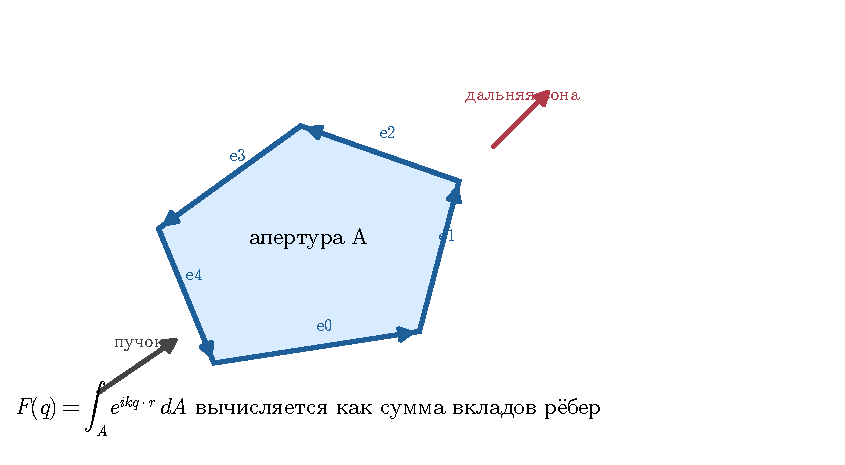
\includegraphics[width=0.84\linewidth]{manual_aperture_edge_ru.pdf}
  \caption{Интеграл по апертуре сводится к сумме вкладов рёбер полигона. Такой
  способ быстрее и точнее прямого численного интегрирования по площади.}
\end{figure}

\subsection{Переход к ребрам полигона}

В системе апертуры:
\[
  A_q=\vect q\cdot\vect h_b,\qquad
  B_q=\vect q\cdot\vect v_b.
\]
Для вершины $j$:
\[
  \Phi_j=k(A_q x_j+B_q y_j).
\]
Если ребро описано через $y=m_jx+c_j$, то один из вариантов суммы по рёбрам имеет вид
\[
  S_x =
  \frac{1}{B_q}
  \sum_{j}
  \frac{\exp(\ii\Phi_{j+1})-\exp(\ii\Phi_j)}
       {A_q+m_jB_q}.
\]
Если удобнее параметризовать ребро как $x=\mu_jy+\eta_j$, используется симметричная форма
\[
  S_y =
  -\frac{1}{A_q}
  \sum_{j}
  \frac{\exp(\ii\Phi_{j+1})-\exp(\ii\Phi_j)}
       {A_q\mu_j+B_q}.
\]
В коде выбор между ветками зависит от того, какой знаменатель устойчивее. Для малых $A_q$ и $B_q$ используется предельная формула площади:
\[
  F_b(\vect 0)\approx C_k\,|A_b|,
\]
где $C_k$ --- комплексный нормировочный множитель, соответствующий выбранной форме интеграла в коде.

\begin{longtable}{L{0.18\linewidth} L{0.72\linewidth}}
\caption{Обозначения в интеграле по рёбрам.}\\
\toprule
Символ & Смысл \\
\midrule
\endfirsthead
\toprule
Символ & Смысл \\
\midrule
\endhead
$\vect q$ & Разность направления пучка и направления наблюдения. \\
$A_q,B_q$ & Компоненты $\vect q$ в плоскости апертуры. \\
$(x_j,y_j)$ & Вершина полигона пучка в системе апертуры. \\
$m_j,\mu_j$ & Наклоны ребра: $dy/dx$ и $dx/dy$. \\
$\Phi_j$ & Фаза комплексной экспоненты в вершине $j$. \\
$S_x,S_y$ & Две эквивалентные формы суммы по рёбрам, выбираемые по устойчивости. \\
\bottomrule
\end{longtable}

\subsection{Почему важны точки 0 и 180 градусов}

В направлениях точно вперёд и точно назад часть базисов и знаменателей
становится вырожденной или почти вырожденной:
\[
  \norm{\vect v_f\times\vect s}\to0,
  \qquad
  A_q\to0,\quad B_q\to0.
\]
Поэтому в этих точках особенно важны:
\begin{itemize}[leftmargin=1.4em]
  \item одинаковая обработка концов углового диапазона на CPU и GPU;
  \item одинаковая формула предела интеграла по рёбрам;
  \item одинаковый вес $\gamma$ на полюсах по $\beta$ при \code{--pole};
  \item отсутствие расхождения в знаке коэффициентов Френеля и в соглашении о
    фазе;
  \item одинаковая точность: одинарная точность может заметно отличаться от
    двойной именно в почти вырожденных ветвях.
\end{itemize}

\subsection{Поглощение}

Если $\Imag(m)>0$ или указан \code{--abs}, внутренняя часть пучка получает затухание:
\[
  \exp(\ii k m L)
  =
  \exp(\ii k \Real(m)L)\,
  \exp(-k\Imag(m)L).
\]
Тогда вклад длинных внутренних путей уменьшается. В численном смысле это помогает сходимости дерева лучей, но меняет физическую интенсивность и поляризационные элементы.

\section{Обрезка пучков в невыпуклых частицах и агрегатах}

\subsection{Затенение апертуры другими гранями}

Для выпуклой частицы пересечение пучка с ближайшей гранью обычно однозначно.
У невыпуклой частицы другая грань может закрывать часть апертуры. Тогда из
полигона текущего пучка вычитают проекцию блокирующей грани:
\[
  P_{\mathrm{vis}}
  =
  P_{\mathrm{subj}}
  \setminus
  \bigcup_{m=1}^{N_c}
  \Pi_{\mathrm{subj}}(C_m).
\]

\begin{figure}[htbp]
  \centering
  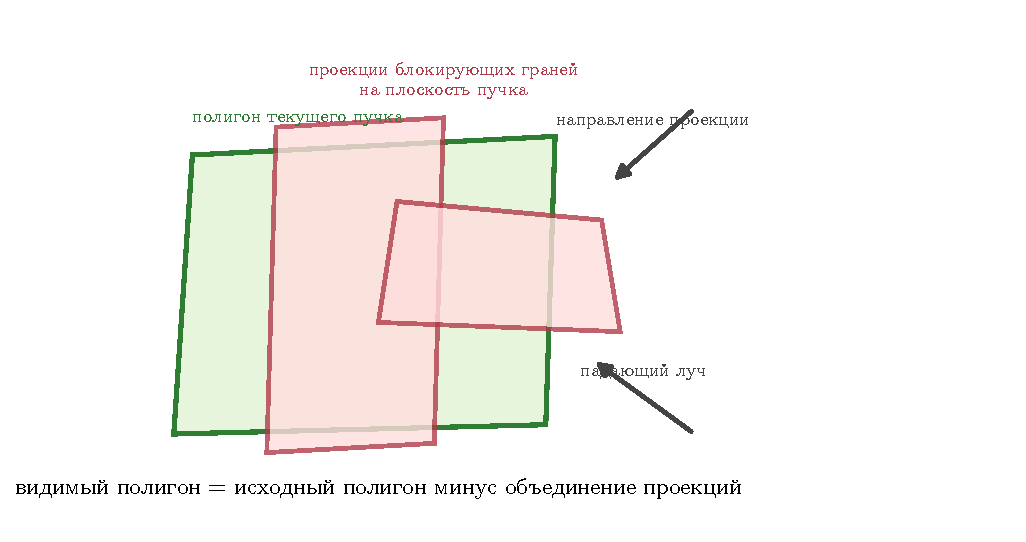
\includegraphics[width=0.82\linewidth]{manual_nonconvex_clipping_ru.pdf}
  \caption{Обрезка невыпуклого пучка: проекция блокирующей грани удаляет
  закрытую часть его полигона.}
\end{figure}

\begin{longtable}{L{0.22\linewidth} L{0.68\linewidth}}
\caption{Объекты геометрической обрезки.}\\
\toprule
Символ & Смысл \\
\midrule
\endfirsthead
\toprule
Символ & Смысл \\
\midrule
\endhead
$P_{\mathrm{subj}}$ & Полигон текущего пучка, который проверяется на видимость. \\
$C_m$ & Блокирующая грань или полигон, потенциально закрывающие текущий пучок. \\
$\Pi_{\mathrm{subj}}$ & Проекция блокирующего объекта на плоскость текущего пучка вдоль направления распространения. \\
$P_{\mathrm{vis}}$ & Видимая часть полигона после вычитания проекций. \\
$N_c$ & Число кандидатов после быстрых фильтров. \\
\bottomrule
\end{longtable}

\subsection{Агрегаты}

В агрегате блокирующая грань может принадлежать другой компоненте:
\[
  C_m \in
  \bigcup_{p=1}^{N_{\mathrm{part}}}
  \mathcal F_p,
\]
где $\mathcal F_p$ --- множество граней компоненты $p$.

\begin{figure}[htbp]
  \centering
  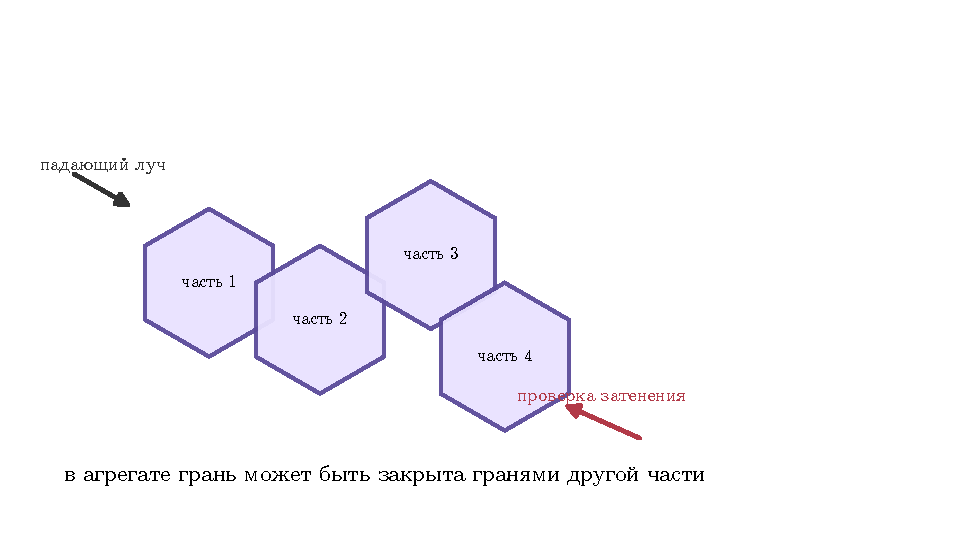
\includegraphics[width=0.82\linewidth]{manual_aggregate_clipping_ru.pdf}
  \caption{Для агрегата затенение идет не только внутри одной компоненты, но и между разными компонентами.}
\end{figure}

\subsection{Предварительный отбор по проекциям AABB}

Точное вычитание полигонов требует значительных затрат. Поэтому
\code{--trace-prefilter} сначала строит ограничивающий прямоугольник проекции
блокирующей грани:
\[
  B(C_m)=
  [x_{\min},x_{\max}]\times[y_{\min},y_{\max}].
\]
Если
\[
  B(C_m)\cap B(P_{\mathrm{subj}})=\varnothing,
\]
то точная обрезка не нужна. Это не меняет физику, а только уменьшает число
дорогих геометрических операций.

\FloatBarrier
\section{Размер частицы и масштабирование геометрии}

В этом разделе различаются геометрические размеры, задаваемые генератору, и
производные характеристики, используемые для сопоставления частиц. Масштаб
всегда применяется к фактически построенной или прочитанной геометрии.

\subsection{Встроенные частицы и геометрия из файла}

Частица задаётся либо параметром \code{--particle}, после которого следуют тип
и его параметры, либо параметром \code{--particle-file} с именем файла. В
первом случае геометрию создаёт встроенный генератор, во втором она читается из
файла. Одновременное задание двух источников запрещено. Параметр
\code{--save-geometry FILE} сохраняет
фактически использованную геометрию после масштабирования и определения её
выпуклости; затем расчёт продолжается.

Координаты файловой частицы и вся внутренняя геометрия трассировки хранятся в
двойной точности. Загрузчик сдвигает координаты относительно не зависящего от
порядка центра ограничивающего параллелепипеда и удаляет только относительный к
масштабу шум текстовой сериализации. Глобальный перенос меняет лишь общую
оптическую фазу; каноническая форма сохраняет матрицу Мюллера, малые рёбра и
порядок граней при больших абсолютных координатах.

\begin{longtable}{L{0.12\linewidth} L{0.30\linewidth} L{0.48\linewidth}}
\caption{Основные встроенные частицы.}\\
\toprule
Тип & Форма & Параметры \\
\midrule
\endfirsthead
\toprule
Тип & Форма & Параметры \\
\midrule
\endhead
1 & Гексагональный столбик или пластинка & \code{L D}: осевая длина и диаметр между
противоположными вершинами. Отношение $L/D$ определяет вытянутую или сплюснутую форму. \\
2 & Пуля & \code{L D}: полная осевая длина и диаметр; высота пирамидальной
головки вычисляется из фиксированного угла $62^\circ$. \\
3 & Розетка из пуль & \code{L D [CAP]}: шесть одинаковых ветвей; без \code{CAP}
используется та же конструкция $62^\circ$. \\
4 & Дрокстал & \code{SCALE}: масштаб фиксированного шаблона; старая форма
\code{L D SCALE} принимает, но игнорирует \code{L,D}. \\
10 & Полый гексагональный столбик & \code{L D CAVITY\_DEG}: верхняя и нижняя
пирамидальные полости; угол должен быть положительным и меньше
$\arctan(L/D)$. \\
12 & Двухкомпонентный гексагональный агрегат & \code{L D 2}: ровно две
одинаковые восьмигранные колонки в фиксированном взаимном положении. \\
999 & Встроенный контрольный агрегат & \code{SCALE}: масштаб фиксированной
регрессионной геометрии. \\
\bottomrule
\end{longtable}

\begin{figure}[htbp]
  \centering
  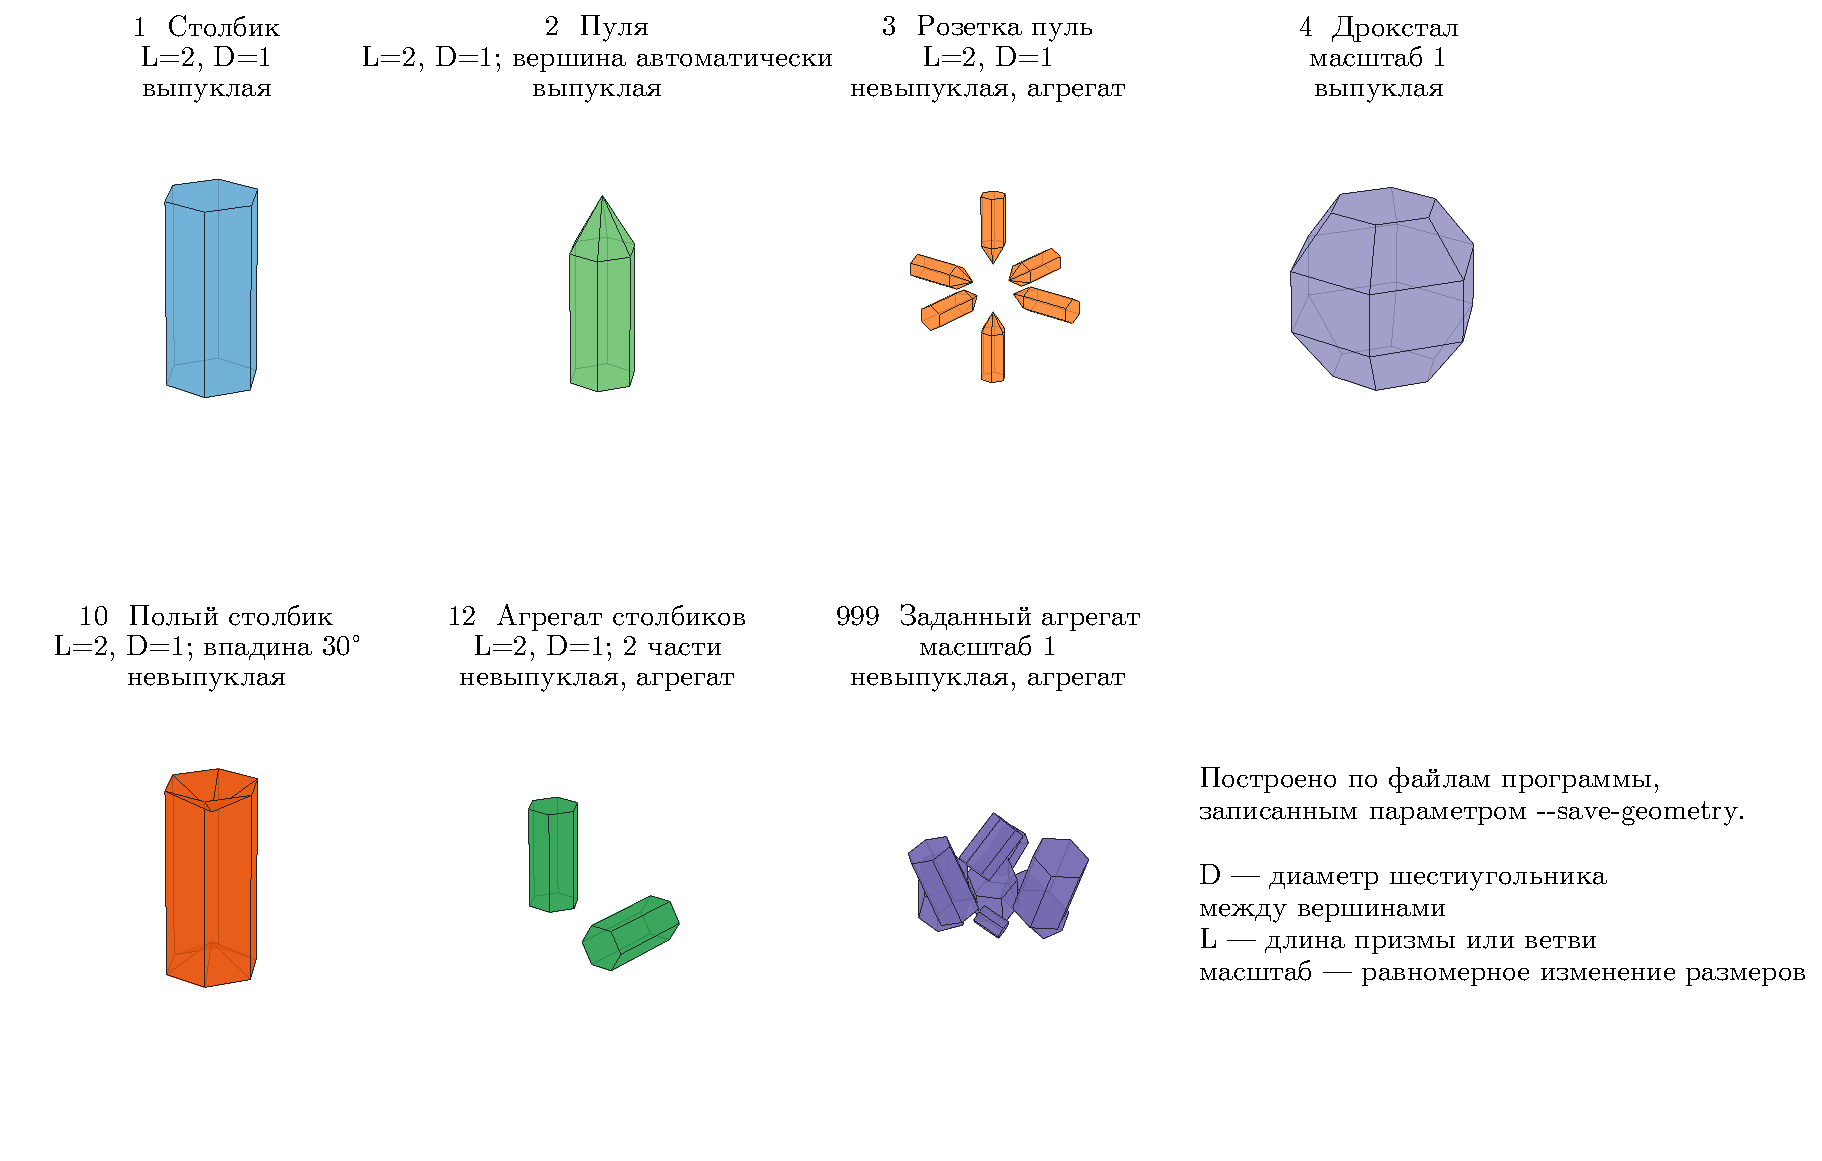
\includegraphics[width=0.98\linewidth]{manual_particle_gallery_ru.pdf}
  \caption{Встроенные формы. Изображения построены по файлам из каталога
  \code{examples/particles}, записанным генераторами самой программы.}
  \label{fig:particle-gallery-ru}
\end{figure}

\subsection{Внутренний формат частицы и экспорт геометрии}

Первые три непустые строки имеют строгий смысл:

\begin{lstlisting}
CONCAVE
AGGREGATE [FACETS_PER_PART]
BETA_DOMAIN_DEG GAMMA_DOMAIN_DEG

x0 y0 z0
x1 y1 z1
x2 y2 z2

x0 y0 z0      # следующая грань
...
\end{lstlisting}

\code{CONCAVE} равен 0 или 1. \code{AGGREGATE} равен 0 для одной частицы
либо записывается как \code{1 FACETS_PER_PART} для компонентов с одинаковым
числом граней. Третья строка задаёт ширину фундаментальной области по $\beta$
и $\gamma$ в градусах. Пустая строка разделяет грани; у каждой грани должно
быть не меньше трёх конечных неколлинеарных вершин. Символ \code{#} начинает
комментарий. Порядок вершин определяет направление нормали, поэтому обход всех
граней должен быть согласован и задавать внешние нормали. Каждая грань должна
быть простым плоским выпуклым многоугольником, а каждая компонента частицы ---
замкнутой многообразной поверхностью. Допускается не более 64 вершин в грани и
256 граней в частице; эти условия проверяются до трассировки.

Экспорт записывает координаты с 17 значащими цифрами и проверяет метаданные
агрегата. Файл содержит уже масштабированную рабочую геометрию, поэтому
подходит для точного повторения расчёта, визуализации обрезки пучков и проверки
цикла «запись--чтение»:

\begin{lstlisting}
gpu/bin/mbs_po_gpu_double --method po \
  --particle 10 20 12 15 \
  --save-geometry concave.particle ...
gpu/bin/mbs_po_gpu_double --method po \
  --particle-file concave.particle ...
\end{lstlisting}

Экспорт состоит из \code{FILE} и \code{FILE.visibility}. Боковой файл хранит
два флага видимости каждой грани и автоматически читается вместе с геометрией.
Для точного повторения расчёта вогнутой встроенной частицы нужны оба файла.
Рабочая геометрия не записывается автоматически; её следует явно сохранить
параметром \code{--save-geometry FILE} (алиас \code{--save-particle}).

\subsection{Эквивалентный радиус и \texorpdfstring{$k_{\mathrm{eq}}$}{k eq}}

Эквивалентный радиус по объему:
\[
  r_{\mathrm{eq}}=
  \left(\frac{3V}{4\pi}\right)^{1/3}.
\]
Эквивалентный размерный параметр:
\[
  k_{\mathrm{eq}}=\frac{2\pi r_{\mathrm{eq}}}{\lambda}.
\]
Если частица масштабируется параметром \code{--k-eq X}, то масштаб $s$ выбирается из
\[
  s =
  \frac{k_{\mathrm{eq,target}}\lambda}{2\pi r_{\mathrm{eq,old}}}.
\]

\begin{longtable}{L{0.18\linewidth} L{0.72\linewidth}}
\caption{Флаги размера.}\\
\toprule
Флаг & Смысл \\
\midrule
\endfirsthead
\toprule
Флаг & Смысл \\
\midrule
\endhead
\code{--resize-dmax-um SIZE} & Масштабировать геометрию из файла так, чтобы $D_{\max}=\code{SIZE}$. \\
\code{--k-eq X} & Масштабировать так, чтобы $k_{\mathrm{eq}}=X$. Требуется \code{--wavelength-um}. \\
\code{--dmax-grid A B N} & Логарифмический диапазон $D_{\max}$. \\
\code{--k-eq-grid A B N} & Логарифмический диапазон $k_{\mathrm{eq}}$. \\
\code{--k-eq-list FILE} & Точный список положительных $k_{\mathrm{eq}}$ из файла. \\
\bottomrule
\end{longtable}

\part{Ориентации и угловые сетки}

\section{Ориентационное усреднение}

\subsection{Интеграл по ориентациям}

Для случайно ориентированных частиц полная средняя по группе вращений имеет
меру
\[
  \langle\matr M\rangle=
  \frac{1}{8\pi^2}
  \int_0^{2\pi}\!\int_0^\pi\!\int_0^{2\pi}
  \matr M(\alpha,\beta,\gamma)
  \sin\beta\,\dd\alpha\,\dd\beta\,\dd\gamma.
\]
В основной двухугловой схеме MBS-fast интеграл по лабораторному углу
$\alpha$ реализован через азимутальную сетку рассеяния. После этого явно
усредняются $\beta$ и $\gamma$:
\[
  \overline{\matr M}(\theta)
  =
  \frac{1}{W}
  \sum_{i=1}^{N_{\mathrm{ori}}}
  w_i\,\matr M_i(\theta),
  \qquad
  W=\sum_{i=1}^{N_{\mathrm{ori}}}w_i.
\]
В непрерывной форме редуцированная двухугловая часть равна
\[
  \overline{\matr M}(\theta)
  =
  \frac{1}{4\pi}
  \int_0^{2\pi}\int_0^{\pi}
  \matr M(\theta;\beta,\gamma)
  \sin\beta\,\dd\beta\,\dd\gamma.
\]
Удобная переменная $\mu=\cos\beta$ дает
\[
  \sin\beta\,\dd\beta=-\dd\mu,
\]
поэтому квадратура по $\mu$ естественным образом учитывает сферическую меру.
Эта формула применима после усреднения по $\alpha$; сама по себе сетка
$\beta\times\gamma$ не заменяет произвольную трёхугловую квадратуру.

\subsection{Регулярная сетка по \texorpdfstring{$\beta,\gamma$}{beta, gamma}}

Если ячейка по $\beta$ имеет границы $\beta_{j-1/2}$ и
$\beta_{j+1/2}$, её вес равен
\[
  w_\beta(j)=
  \cos\beta_{j-1/2}-\cos\beta_{j+1/2}.
\]
Для равномерной сетки по $\gamma$
\[
  w_\gamma=\frac{\gamma_{\max}-\gamma_{\min}}{N_\gamma}.
\]
Итоговый вес:
\[
  w_{j,l}=w_\beta(j)w_\gamma(l).
\]

\subsection{Флаг \texorpdfstring{\code{--pole}}{--pole}}

На полюсах $\beta=0$ и $\beta=\pi$ все $\gamma$ описывают одну и ту же
физическую ориентацию:
\[
  \matr R_z(\gamma)\matr R_y(0)=\matr R_z(\gamma),
\]
Поэтому \code{--pole} оставляет на полюсе одну точку по $\gamma$, но назначает
ей вес всего интервала:
\[
  w_{\mathrm{pole}}=w_\beta\,(\gamma_{\max}-\gamma_{\min}).
\]
Эту специальную ветвь необходимо одинаково реализовывать на CPU и GPU.
Расхождение полюсного веса или выбора базиса прежде всего проявляется в
направлениях $0^\circ$ и $180^\circ$.

\subsection{Сетка по дифракционной оценке}

Канонический параметр \code{--diffraction-sampling Q} строит сетки ориентаций
и направлений рассеяния из одной оценки дифракционного углового масштаба:
\[
  \xi
  =
  0.69\,\frac{\lambda}{l_{\max}}.
\]
Здесь $\xi$ выражена в радианах, а $l_{\max}$ --- максимальная длина ребра
среди всех граней уже масштабированной частицы:
\[
  l_{\max}=\max_f\max_i
  \left\lVert\vect r_{f,i+1}-\vect r_{f,i}\right\rVert,
  \qquad \vect r_{f,n_f}=\vect r_{f,0}.
\]
Это не диаметр частицы и не максимальное расстояние между произвольными
вершинами. Параметр $Q$ задаёт число угловых интервалов на масштабе $\xi$:
\[
  \Delta_{\mathrm{target}}=\frac{\xi}{Q}.
\]
Следовательно, $Q=1$ соответствует шагу $\xi$, $Q=2$ --- шагу $\xi/2$, а
$Q=4$ --- шагу $\xi/4$. Чем больше $Q$, тем мельче сетка и дороже расчёт.
Число $Q$ не является общим числом ориентаций или числом точек на кольце.

\begin{center}
\begin{minipage}{0.90\linewidth}
  \centering
  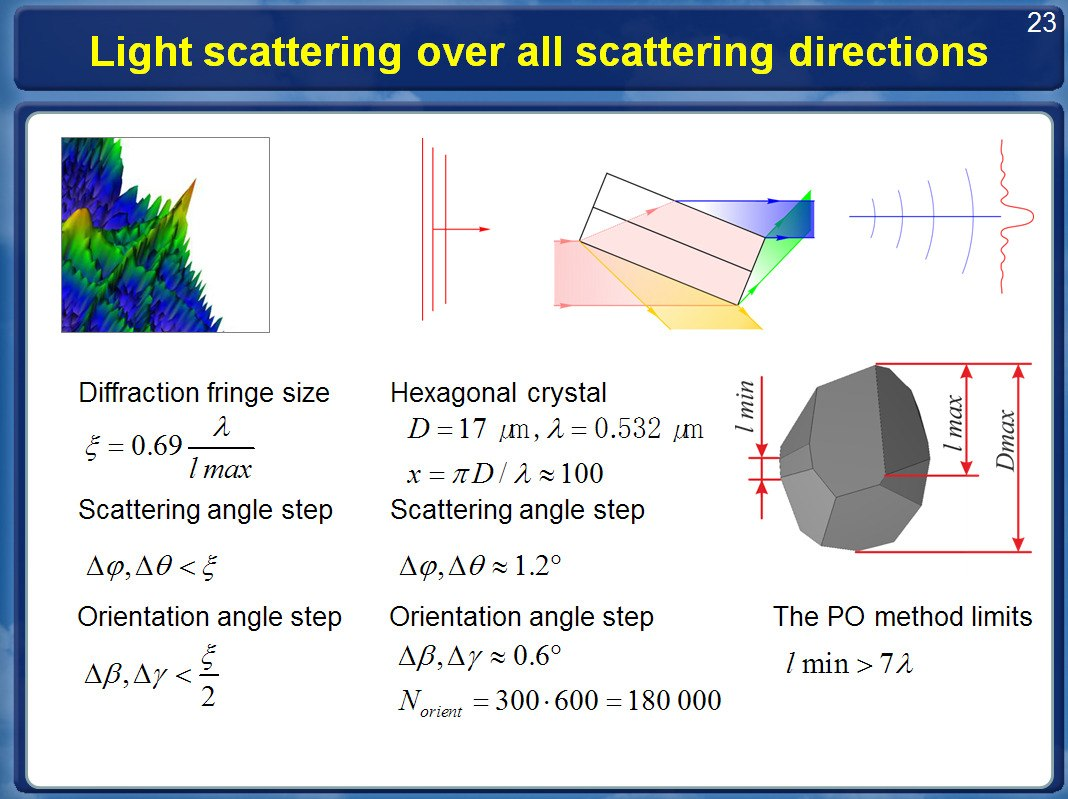
\includegraphics[width=\linewidth]{diffraction_sampling_estimate.jpeg}
  \captionof{figure}{Исходная оценка углового разрешения по дифракционной
  полосе. Показанное условие $\Delta\phi,\Delta\theta<\xi$ соответствует
  $Q_{\mathrm{scat}}\geq1$, а
  $\Delta\beta,\Delta\gamma<\xi/2$ --- $Q_{\mathrm{ori}}\geq2$.
  В программе $l_{\max}$ вычисляется как максимальная длина ребра среди всех
  граней частицы, отдельно от полного диаметра $D_{\max}$.}
  \label{fig:diffraction-sampling-estimate}
\end{minipage}
\end{center}

Для ориентаций программа вычисляет
\[
  N_\beta=\max\!\left(3,
    \left\lceil\frac{\beta_{\max}-\beta_{\min}}{\xi/Q_\mathrm{ori}}\right\rceil
  \right),\qquad
  N_\gamma=\max\!\left(3,
    \left\lceil\frac{\gamma_{\max}-\gamma_{\min}}{\xi/Q_\mathrm{ori}}\right\rceil
  \right).
\]
Фундаментальные диапазоны $\beta$ и $\gamma$ берутся из симметрии частицы;
\code{--mirror-gamma} дополнительно сокращает область по $\gamma$. Из-за
округления фактические шаги могут быть немного меньше целевого $\xi/Q$.

Общий флаг назначает $Q_\mathrm{ori}=Q_\mathrm{scat}=Q$. Если требуется
другая плотность только для ориентаций, применяется переопределение
\code{--orientation-diffraction-sampling Q}. Например,
\begin{lstlisting}[language=bash]
--diffraction-sampling 2 \
--orientation-diffraction-sampling 4
\end{lstlisting}
задаёт $\xi/4$ для $\beta,\gamma$ и сохраняет $\xi/2$ для $\theta,\phi$.
Параметр \code{--orientation-diffraction-sampling} можно использовать без
общего флага и совместить с явно заданным \code{--scattering-grid}.

Исторические параметры \code{--diffraction-grid},
\code{--diffraction-limit-grid} и \code{--ring-points} сохранены только для
совместимости старых команд и показаны в \code{--help-debug}. Их нельзя
смешивать с новой схемой: прежний алгоритм использовал другую зависимость
числа ориентаций от делителя и скрытое значение \code{ring-points=3}.
Расчёты, выполненные до исправления определения $l_{\max}$, могли строить
сетку по диаметру частицы; повторный запуск такой команды в новой версии
правильно использует максимальное ребро и поэтому может выбрать другое число
ориентаций.

\subsection{Квазислучайные и случайные выборки}

Квазислучайные режимы заменяют регулярную сетку набором точек низкой дискрепантности. Идея:
\[
  \overline{\matr M}_N
  =
  \frac1N\sum_{i=1}^{N}
  \matr M(T(\vect u_i)),
\]
где $\vect u_i\in[0,1)^d$ --- Sobol/Hammersley/lattice point, а $T$ переводит единичный куб в углы ориентации с правильной мерой.

\begin{longtable}{L{0.22\linewidth} L{0.68\linewidth}}
\caption{Ориентационные методы.}\\
\toprule
Флаг & Метод \\
\midrule
\endfirsthead
\toprule
Флаг & Метод \\
\midrule
\endhead
\code{--fixed-orientation B G} & Одна ориентация $\beta,\gamma$ в градусах; удобна для отладки CPU/GPU. \\
\code{--orientation-file FILE} & Пары $\beta,\gamma$ в градусах, по одной паре на строку. \\
\code{--euler-grid NB NG} & Явная регулярная сетка $\beta\times\gamma$. \\
\flag{--diffraction-sampling} \code{Q} & Регулярная сетка ориентаций и автоматическая сетка рассеяния с шагом $\xi/Q$. \\
\flag{--orientation-diffraction-sampling} \code{Q} & Только регулярная сетка ориентаций с шагом $\xi/Q$. \\
\code{--sobol N} & Квазислучайная последовательность Соболя. \\
\code{--sobol-seed N SEED} & Последовательность Соболя с заданным перемешиванием Оуэна. \\
\code{--so3-quaternion N} & Хаммерсли в области симметрии; лабораторный $\alpha$ интегрируется по азимуту рассеяния. \\
\code{--so3-mirror-audit} & При чётном $N$ явно трассировать вложенные отражённые пары для проверки \flag{--mirror-gamma}. \\
\code{--so3-full-quaternion N} & Прямая выборка полной группы $SO(3)$ через кватернионы Шумейка для независимой проверки. \\
\code{--hammersley N} & Выборка Хаммерсли. \\
\code{--lattice N} & Ранговая решётка первого порядка. \\
\code{--monte-carlo N} & Псевдослучайные ориентации; ошибка обычно убывает как $N^{-1/2}$. \\
\bottomrule
\end{longtable}

\subsection{Квадратура SO(3) с учетом симметрии}

Для изотропного ансамбля мера Хаара в принятом соглашении углов равна
\[
 dR \mathrel{\propto} \sin\beta\,d\beta\,d\gamma\,d\alpha.
\]
Режим \code{--so3-quaternion N} использует фундаментальную область частицы
$0\leq\beta\leq\beta_{\mathrm{sym}}$,
$0\leq\gamma<\gamma_{\mathrm{sym}}$. Для $i=0,\ldots,N-1$ строятся узлы
\[
 u_i=\frac{i+1/2}{N},\qquad
 v_i=\operatorname{radical\_inverse}_2(i),
\]
\[
 \beta_i=\arccos\!\left[1-(1-\cos\beta_{\mathrm{sym}})u_i\right],\qquad
 \gamma_i=\gamma_{\mathrm{sym}}v_i,\qquad w_i=\frac1N.
\]
Равномерно распределён $\cos\beta$, а не сам $\beta$; нормированные веса
удовлетворяют $\sum_i w_i=1$. Флаг \code{--sym Sb Sg} переопределяет область:
$\beta_{\mathrm{sym}}=\pi/S_b$,
$\gamma_{\mathrm{sym}}=2\pi/S_g$. Его допустимо использовать только при
реальной симметрии геометрии.

Для парной проверки зеркальной реконструкции к чётному полному числу узлов
добавляется \code{--so3-mirror-audit}. При $K=N/2$ те же формулы применяются
для $i=0,\ldots,K-1$ с $u_i=(i+1/2)/K$ и
$\gamma_i=(\gamma_{\mathrm{sym}}/2)v_i$, после чего явно трассируются пары
$(\beta_i,\gamma_i)$ и $(\beta_i,\gamma_{\mathrm{sym}}-\gamma_i)$ с весом
$1/N$. Эта сетка точно вложена в расчёт из $K$ узлов с
\flag{--mirror-gamma}. Без контрольного флага обычная полнодоменная
последовательность Хаммерсли не меняется.

С флагом \flag{--mirror-gamma} вычисляется только диапазон
$0\leq\gamma<\gamma_{\mathrm{sym}}/2$. Вторая половина восстанавливается до
квадратуры по $\alpha$:
\[
 \matr M_{\mathrm{full}}(\theta,\phi)=\frac12\left[
 \matr M_{\mathrm{half}}(\theta,\phi)
 +\matr P\matr M_{\mathrm{half}}(\theta,-\phi)\matr P\right],\qquad
 \matr P=\operatorname{diag}(1,1,-1,-1).
\]
Преобразование допустимо только при наличии у всей оптической частицы
соответствующей плоскости отражения, включая видимость граней и назначенные
материалы, а также при численной инвариантности выбранного трассировщика ФО
относительно такого отражения. По одному файлу частицы программа не может
доказать это свойство; для каждого нового класса частиц и набора параметров
нужен контрольный расчёт с полным диапазоном $\gamma$. $N$ остаётся числом
реально трассируемых ориентаций $\beta,\gamma$. Для строгой парной проверки
сравниваются \code{--so3-quaternion 4096 --so3-mirror-audit} и
\code{--so3-quaternion 2048 --mirror-gamma}. Их базовые узлы совпадают, поэтому
разность измеряет численную ошибку зеркальной реконструкции, а не шум двух
разных выборок Хаммерсли. Обычную полнодоменную сетку также надо сравнить с
независимым плотным результатом, а обратное рассеяние проверить отдельно.

Угол $\alpha$ отдельно не трассируется. Поворот вокруг падающего луча
эквивалентен изменению азимута рассеяния $\phi$, поэтому каждая строка
$\theta$ накапливается как
\[
 \overline{M}(\theta)=\frac{1}{N_\phi}
 \sum_{\phi}M(\theta,\phi)L(-\phi).
\]
Матрица $L$ поворачивает базис Стокса; её блок $Q/U$ содержит
$\cos(2\phi)$ и $\sin(2\phi)$. Умножение выполняется справа, поскольку
меняется базис падающей поляризации. В направлениях $\theta=0$ и $\theta=\pi$
азимутальный базис вырожден: код усредняет без $L$, затем накладывает точную
форму матрицы для прямого или обратного направления.

Режим требует $N_\phi\geq2$. Для итогового запуска его следует сочетать с
\flag{--scattering-diffraction-sampling} \code{Q} и
\flag{--latitude-phi-grid}. Более медленный
\flag{--so3-full-quaternion} \code{N} нужен только для проверки:
там $N$ означает число полных трёхмерных поворотов, а в быстром режиме $N$ ---
число действительно трассируемых ориентаций $\beta,\gamma$; квадратуру по
$\alpha$ выполняет сетка $\phi$.

\subsection{Адаптивный выбор числа ориентаций}

При сравнении кандидатов по $N_\phi$, глубине отражений и сетке Эйлера
для двух приближений $A$ и $B$ ошибка одной строки по $\theta$ равна
\[
e_{\mathrm{row}}=
\max\!\left(
\frac{|M^{A}_{11}-M^{B}_{11}|}
{\max(|M^{A}_{11}|,|M^{B}_{11}|,\varepsilon_0)},
\max_{(i,j)\ne(1,1)}
\frac{|R^{A}_{ij}-R^{B}_{ij}|}
{\max(1,|R^{A}_{ij}|,|R^{B}_{ij}|)}
\right),
\qquad
R_{ij}=\frac{M_{ij}}{M_{11}}.
\]
Здесь $R_{ij}=M_{ij}/M_{11}$, а $\varepsilon_0$ защищает деление около
нулей. Затем берётся максимум по строкам $\theta$ и добавляется относительное
изменение интеграла $\int M_{11}\,\dd\Omega$. Для глубины отражений также
проверяется выходная энергия. При подборе сетки $\theta$ значения в точках
$1/3$ и $2/3$ каждого интервала сравниваются с интерполяцией, после чего
отдельно проверяется интеграл $M_{11}$. При подборе числа точек Соболя
проверяются входная энергия и все 16 элементов на контрольных углах.

По умолчанию для числа ориентаций, $N_\phi$, глубины отражений и сетки Эйлера
требуются два последовательных успешных уточнения; сетка $\theta$ уточняет
интервалы напрямую. Параметр \code{--convergence-passes N} меняет число таких
подтверждений. В совместных адаптивных режимах достижение верхнего предела
считается ошибкой. Отдельный режим \code{--adaptive-orientations} выдаёт
предупреждение и сохраняет лучший результат, но не подтверждает сходимость.

\subsection{Файл настроек адаптивной сходимости}

Параметр \code{--adaptive-config FILE} загружает все пределы рабочего расчёта из одного
текстового файла. Полный шаблон с пояснением каждой строки находится в файле
\nolinkurl{configs/adaptive.example.conf}. Формат строгий: \code{key = value}; после
символа \texttt{\#} или \texttt{;} разрешен комментарий. Например:

\begin{lstlisting}
reflections.min = 2
reflections.max = 30
reflections.tolerance = 0.01  # 1 percent
alpha.min_points = 12
alpha.max_points = 2400
alpha.tolerance = 0.01
orientations.min = 128
orientations.max = 262144
orientations.tolerance = 0.02
\end{lstlisting}

Группы \code{reflections}, \code{alpha}, \code{theta},
\code{orientations}, \code{beta} и \code{gamma} задают минимум, максимум и
свою относительную точность. Группа \code{controller} задает число
последовательных успешных уточнений, диапазон pilot-набора и максимальное число
совместных проходов. Значение \code{0.01} означает относительную погрешность
1\%, а не 0.01\%.

Если индивидуальная точность отсутствует в файле, используется общий
\code{EPS} из \code{--auto}, \code{--autofull} или другого выбранного режима.
Индивидуальная точность из файла имеет приоритет над общим \code{EPS}. Явные
флаги командной строки \code{--max-*}, \code{--max-reflections} и
\code{--convergence-passes} имеют приоритет над файлом. Неизвестный или
повторный ключ, неверный диапазон и неправильный тип значения останавливают
запуск до расчета с указанием файла, номера строки и способа исправления.

\begin{lstlisting}
cpu/bin/mbs_po_mpi --method po --particle 1 100 70 \
  --refractive-index 1.3116 0 --wavelength-um 0.532 \
  --autofull 0.02 \
  --adaptive-config configs/adaptive.example.conf \
  --backend cpu --threads 64 --output converged --close
\end{lstlisting}

\subsection{Совместный адаптивный подбор параметров}

Параметры не являются независимыми. Глубина $n$ меняет дерево лучей;
$N_\phi$ меняет эквивалентное усреднение по $\alpha$; сетка $\theta$
определяет, на каких углах контролируется результат; число ориентаций меняет
каждую усреднённую строку. Поэтому общий порядок имеет вид
\[
n\longrightarrow N_\phi\longrightarrow
\{\theta_j\}\longrightarrow N_{\mathrm{orient}}.
\]
\code{--auto EPS} оставляет $n$ фиксированным и подбирает $N_\phi$, сетку
$\theta$ и число точек Соболя. \code{--autofull EPS} дополнительно подбирает
$n$. \code{--diffraction-autofull EPS} завершает поиск регулярной квадратурой
Эйлера: $N_\beta$ и $N_\gamma$ уточняются по очереди, затем проверяются
совместно. Цикл повторяется на увеличенном контрольном наборе, пока выбранные
параметры не перестанут изменяться.

В совместном автоматическом режиме параметр \code{--phi-points N} фиксирует
$N_\phi$. Параметры \code{--scattering-grid} и \code{--theta-grid-file}
фиксируют сетку $\theta$;
остальные параметры продолжают подбираться. Чтобы искать эту размерность,
соответствующий явный флаг надо убрать. Отдельные \code{--adaptive-phi} и
\code{--auto-phi} по-прежнему несовместимы с \code{--phi-points}, потому что их
единственная задача --- подобрать $N_\phi$.

\code{--auto-theta-grid EPS} проверяет две внутренние точки каждого интервала
по полной матрице Мюллера и по интегралу $M_{11}$. В алгоритме нет заранее
заданных углов особых областей: особенности конкретной формы должны
обнаруживаться по рассчитанной кривой. Приближённая стоимость равна
\[
  \text{стоимость}\approx
  N_{\mathrm{ori}}\,
  N_{\theta}\,
  N_{\phi}\,
  N_b.
\]
Поэтому автоматический режим может быть заметно дороже одной заранее заданной
сетки, но он даёт измеряемый критерий выбора параметров.

Каждая попытка записывается в файл
\code{<output>/<name>_convergence.tsv}: параметр, номер совместного прохода, кандидат, максимальная ошибка, худший theta-угол, номер элемента и статус.

\subsection{Почему симметрия столбика не делит \texorpdfstring{$N_\phi$}{N phi} на шесть}

В коде используется соглашение
\[
\matr R=R_z(\alpha)R_y(\beta)R_z(\gamma).
\]
Цикл по азимуту рассеяния за счет вращательной ковариантности реализует усреднение по лабораторному углу $\alpha$, поэтому в этом контексте $N_\phi=N_\alpha$. У шестигранного столбика есть осевая симметрия $R_z(2\pi/6)$ в системе частицы. Она уже сокращает область $\gamma$ до
\[
0\leq\gamma<\frac{\pi}{3}=60^\circ.
\]
Но при $\beta\ne0,\pi$ наклоненный столбик не инвариантен относительно поворота на $60^\circ$ вокруг лабораторной оси падающего луча. Поэтому для $\alpha$ остается область $0\leq\alpha<2\pi$, и автоматическое деление $N_\phi$ на шесть было бы физически неверным. \code{--alpha-points} является понятным алиасом \code{--phi-points}, а \code{--adaptive-alpha} --- алиасом \code{--adaptive-phi}; они не включают дополнительное приближение.

\section{Угловая сетка рассеяния}

\subsection{Строки по \texorpdfstring{$\theta$}{theta} и телесный угол}

Равномерная сетка \code{--scattering-grid T0 T1 NPHI NTH} содержит
$N_{\theta}+1$ строк. Вес строки равен
\[
  \Delta\Omega_j=
  2\pi\left[
  \cos\theta_{j,\mathrm{left}}
  -
  \cos\theta_{j,\mathrm{right}}
  \right].
\]
Для полного диапазона $0^\circ\ldots180^\circ$:
\[
  \sum_j\Delta\Omega_j=4\pi.
\]

\subsection{Азимутальная сетка}

В полном расчёте используется $N_\phi$ азимутальных точек. В итоговом файле
для случайных ориентаций обычно записан результат, уже усреднённый по азимуту,
но внутри алгоритма $\phi$ остаётся отдельным измерением работы:
\[
  N_{\mathrm{work}}\sim
  N_b\,N_\theta\,N_\phi\,N_{\mathrm{ori}}.
\]

\subsection{Дифракционная оценка и широтная сетка по \texorpdfstring{$\phi$}{phi}}

В PO-режиме \code{--diffraction-sampling Q} использует для сетки рассеяния
тот же масштаб $\xi_0=0.69\lambda/l_{\max}$, что и для ориентаций. Целевой
шаг равен
\[
  \Delta_{\mathrm{scat}}=\frac{\xi_0}{Q_{\mathrm{scat}}}.
\]
Числа интервалов вычисляются как
\[
  N_\theta=\left\lceil\frac{\pi}{\Delta_{\mathrm{scat}}}\right\rceil,
\]
\[
  N_{\phi,\mathrm{eq}}=
  \operatorname{round\_up}_6\!\left[
    \max\!\left(12,
      \left\lceil\frac{2\pi}{\Delta_{\mathrm{scat}}}\right\rceil\right)
  \right].
\]
Результат содержит $N_\theta+1$ строк от $0$ до $\pi$. Значение $Q=1$
использует дифракционный масштаб непосредственно, а $Q=2$ уменьшает оба
целевых угловых шага вдвое. Это априорная оценка разрешения, а не гарантия
точности. Для итогового расчёта следует сравнить выбранное $Q$ с удвоенным
значением по всем требуемым элементам матрицы Мюллера.

Параметр \code{--scattering-diffraction-sampling Q} переопределяет только
$Q_{\mathrm{scat}}$. Например,
\begin{lstlisting}[language=bash]
--diffraction-sampling 2 \
--scattering-diffraction-sampling 1
\end{lstlisting}
оставляет шаг ориентаций $\xi_0/2$, но задаёт шаг рассеяния $\xi_0$.

Флаг \code{--latitude-phi-grid} сохраняет экваториальное разрешение, но
задает отдельное число азимутальных точек для каждой строки:
\[
  N_\phi(\theta)=\min\!\left\{N_{\phi,\mathrm{eq}},
  \operatorname{round\_up}_6\!\left[
    \max\!\left(12,
      \left\lceil\frac{2\pi\sin\theta}{\Delta_{\mathrm{scat}}}\right\rceil\right)
  \right]\right\}.
\]
Так удаляются почти совпадающие азимутальные направления около полюсов без
огрубления экватора. Число узлов округляется до кратного шести, а полюсная
строка связывается с соседней рабочей группой для устойчивой обработки
  базиса. Накопление выполняется на полной прямоугольной выходной сетке
$N_{\phi,\mathrm{eq}}$, поэтому формат результата не меняется.

Переменная широтная сетка поддерживается как для дифракционной сетки
ориентаций, так и для сокращённого режима \code{--so3-quaternion N}, по одному
размеру частицы на процесс. Для SO(3) предпочтителен параметр
\flag{--scattering-diffraction-sampling} \code{Q}: общий
\flag{--diffraction-sampling} \code{Q} сам задаёт основной регулярный ориентационный
режим. Автоматическая сетка конфликтует с явными \code{--scattering-grid},
\code{--theta-grid-file}, \code{--auto-theta-grid} и \code{--phi-points}.
Широтная сетка пока не поддерживается общим
последовательным расчётом нескольких размеров. Каждый размер следует запускать
отдельным процессом, чтобы
$l_{\max}$ и сетка пересчитывались заново.

\begin{lstlisting}[language=bash]
CUDA_VISIBLE_DEVICES=0,1,2,3 \
MBS_GPU_GROUPS=1 MBS_GPU_MULTI_MAX=4 \
gpu/bin/mbs_po_gpu_double --method po \
  --particle 1 100 70 --refractive-index 1.3116 0 \
  --wavelength-um 0.532 --max-reflections 8 \
  --diffraction-sampling 2 \
  --latitude-phi-grid --backend cuda --threads 32 \
  --output results/column --close
\end{lstlisting}

\subsection{Адаптивная сетка по \texorpdfstring{$\theta$}{theta}}

Передний дифракционный пик обычно требует более мелкого шага, чем боковые и
задние углы. Режим \code{--auto-theta-grid EPS} не использует заранее
назначенные зоны. Он сравнивает рассчитанные значения с интерполяцией в точках
$1/3$ и $2/3$ каждого интервала, уточняет только не прошедшие интервалы и
отдельно контролирует изменение интеграла $M_{11}$. Верхняя граница числа
узлов задаётся параметром \code{--max-theta-points}.

\part{Реализация и производительность}

\section{Реализация на CPU и AVX}

\subsection{Что параллелится на CPU}

В CPU-версии OpenMP и MPI распределяют ориентации, строки сетки $\theta$,
пучки и группы размеров. К наиболее затратным операциям относятся вычисление фаз
\[
  \Phi = k(A_qx+B_qy),\qquad
  \exp(\ii\Phi)=\cos\Phi+\ii\sin\Phi,
\]
суммирование вкладов рёбер и накопление матриц Джонса и Мюллера.

Для регулярной фазы многоугольника CPU-цикл PO обрабатывает четыре соседних
направления $\theta$ одной AVX2-операцией над интегралом по рёбрам. В каждой
векторной полосе сохраняется исходный порядок суммирования рёбер. При малой
фазе или активном почти сингулярном знаменателе вся группа автоматически
переходит на исходную устойчивую скалярную формулу. Режим включён в обычную
CPU-сборку, не требует флага и не вводит новой пользовательской точности.
Временные массивы фазы и синуса/косинуса хранятся сначала по вершине, затем по
соседним направлениям $\theta$. Поэтому AVX2-цикл загружает четыре соседних
значения напрямую вместо сбора из четырёх строк. На представительном тесте
поглощающего вогнутого столбика медианное время уменьшилось с 12,76 до 11,37~с
(в 1,12 раза) относительно предыдущей векторизованной реализации, а таблица
Мюллера совпала побитно.

\subsection{Упаковка данных в AVX-512}

\begin{figure}[htbp]
  \centering
  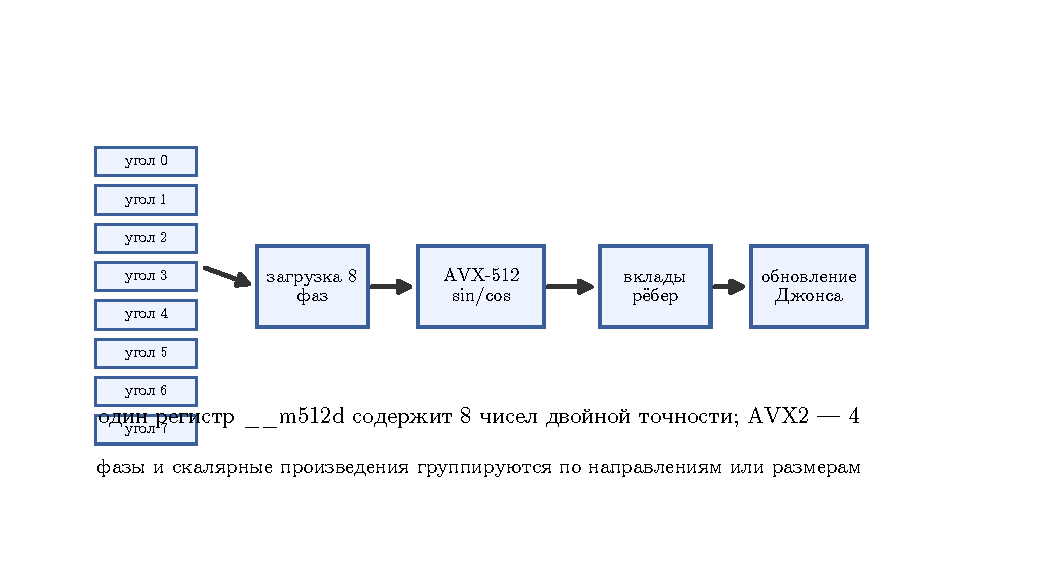
\includegraphics[width=0.92\linewidth]{manual_avx512_packing_ru.pdf}
  \caption{AVX-512 обрабатывает восемь значений двойной точности в одном
  векторном регистре; AVX2 обрабатывает четыре.}
\end{figure}

Для AVX-512 в двойной точности:
\[
  \vect\Phi =
  (\Phi_0,\Phi_1,\ldots,\Phi_7),
\]
\[
  \vect C=\cos\vect\Phi,\qquad
  \vect S=\sin\vect\Phi.
\]
Одна векторная команда или векторизованный полиномиальный алгоритм обрабатывает
сразу восемь направлений наблюдения либо восемь размеров. Для AVX2:
\[
  \vect\Phi_{\mathrm{AVX2}}=(\Phi_0,\Phi_1,\Phi_2,\Phi_3).
\]

\subsection{Почему важны флаги компиляции}

Если компилятор не имеет права генерировать AVX-512, быстрый путь не включится. Для EPYC:
\begin{longtable}{L{0.25\linewidth} L{0.36\linewidth} L{0.29\linewidth}}
\caption{Рекомендуемые CPU-флаги.}\\
\toprule
Платформа & \code{ARCH_FLAGS} & Комментарий \\
\midrule
\endfirsthead
\toprule
Платформа & \code{ARCH_FLAGS} & Комментарий \\
\midrule
\endhead
EPYC Zen2 & \code{-march=znver2 -mtune=znver2} & AVX2/FMA. \\
EPYC Zen3 & \code{-march=znver3 -mtune=znver3} & AVX2/FMA. \\
EPYC Zen4 & \code{-march=znver4 -mtune=znver4} & AVX-512 при поддержке GCC/Clang. \\
EPYC Zen5 & \code{-march=znver5 -mtune=znver5} & Лучший вариант для новых компиляторов. \\
Переносимый AVX2 & \code{-O3 -mavx2 -mfma} & Для переносимого бинарного файла под AVX2. \\
Явный AVX-512 &
\code{-O3 -mavx512f -mavx512dq}\newline
\code{-mavx512cd -mavx512bw -mavx512vl} &
Только если \code{lscpu} показывает эти возможности. \\
\bottomrule
\end{longtable}

Флага \code{AVX12} у GCC/Clang нет. Если имеется в виду EPYC Zen5 с AVX-512, используйте \code{-march=znver5}; если компилятор старый, используйте явные \code{-mavx512*} после проверки \code{lscpu}.

\section{Реализация на GPU}

\subsection{Что ускоряет GPU}

GPU ускоряет дифракционную часть, потому что она раскладывается на почти
независимые элементы работы:
\[
  (b,\theta,\phi,o)\mapsto \matr J_{b,o}(\theta,\phi),
\]
где $b$ --- номер пучка, а $o$ --- номер ориентации. До когерентного
суммирования каждый вклад вычисляется независимо.

\begin{figure}[htbp]
  \centering
  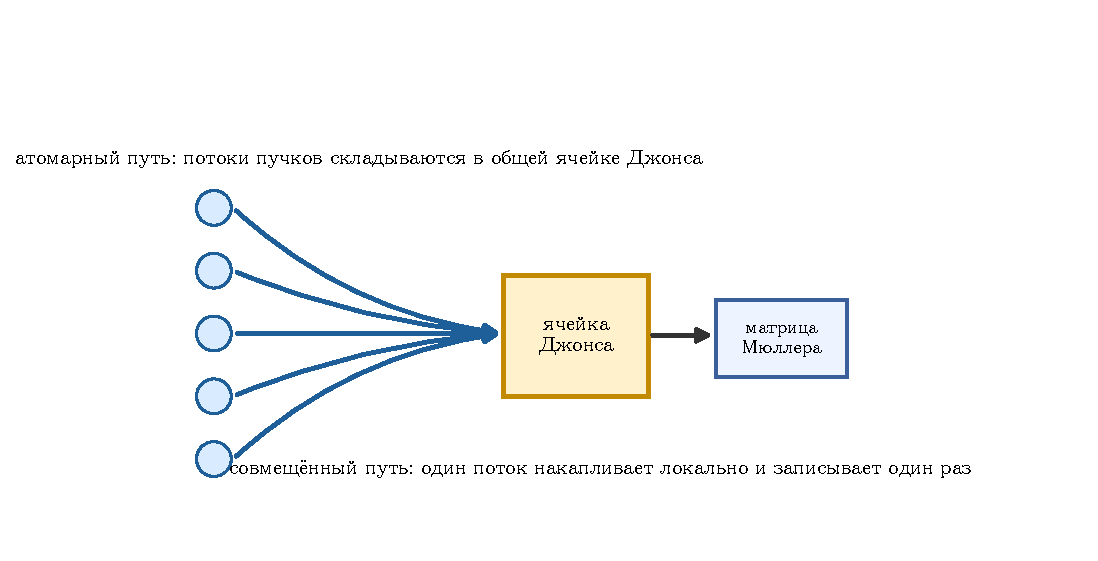
\includegraphics[width=0.92\linewidth]{manual_gpu_atomics_ru.pdf}
  \caption{Варианты CUDA-вычислений: атомарное накопление матриц Джонса,
  владение ячейкой без атомарных операций и совмещённое вычисление дифракции
  с преобразованием в матрицу Мюллера.}
\end{figure}

\begin{longtable}{L{0.23\linewidth} L{0.30\linewidth} L{0.37\linewidth}}
\caption{Основные варианты ядер GPU.}\\
\toprule
Вариант & Работа одного потока & Область применения \\
\midrule
\endfirsthead
\toprule
Вариант & Работа одного потока & Область применения \\
\midrule
\endhead
Атомарное накопление & Вычисляет вклад пучка и добавляет его командой \code{atomicAdd} в матрицу Джонса. & Универсальный резервный и диагностический путь. \\
Владение ячейкой & Один поток владеет выходной ячейкой и последовательно проходит пучки. & Когда размещение данных позволяет избежать конкурирующих записей. \\
Совмещённое ядро & Локально суммирует матрицу Джонса и сразу преобразует её в матрицу Мюллера. & Основной путь при записи только полного результата. \\
Поэтапное накопление & Сначала строит матрицы отдельных ориентаций, затем редуцирует их. & Большие блоки ориентаций и высокая конкуренция атомарных операций. \\
Несколько $k_{\mathrm{eq}}$ & Обрабатывает близкие размеры из общего набора пучков. & Серии размеров с совместимыми геометрией и сеткой. \\
\bottomrule
\end{longtable}

\subsection{Атомарное накопление}

Матрица Джонса имеет четыре комплексных элемента:
\[
  \matr J=
  \begin{pmatrix}
  J_{00}&J_{01}\\
  J_{10}&J_{11}
  \end{pmatrix},
  \qquad
  J_{pq}=x_{pq}+\ii y_{pq}.
\]
Атомарный вариант выполняет восемь сложений:
\[
  \operatorname{atomicAdd}(x_{pq}),\qquad
  \operatorname{atomicAdd}(y_{pq}),\qquad
  p,q\in\{0,1\}.
\]
Это корректно для когерентной суммы, но порядок сложения не детерминирован.
Поэтому младшие разряды могут отличаться от CPU, особенно в одинарной точности
и около вырожденных направлений.

\subsection{Почему совмещённое ядро быстрее}

Совмещённое ядро не записывает полный промежуточный массив матриц Джонса в
глобальную память:
\[
  \sum_b\matr J_b
  \;\longrightarrow\;
  \mathcal M\!\left(\sum_b\matr J_b\right)
  \;\longrightarrow\;
  \text{глобальный массив Мюллера}.
\]
Это уменьшает обмен с глобальной памятью и число атомарных операций, повышая
вычислительную интенсивность. Эффект особенно заметен при больших $N_b$ и
$N_\phi$.

Отдельное ускорение по азимуту даёт интерполяция cuFFT. Для автоматического выбора
используется \code{--fft}, для явного и воспроизводимого сжатия
\code{--fft-factor N}, а для измеряемого контроля на вложенной сетке
\code{--fft-tolerance EPS}. Алгоритм, цена дополнительной проверки и смысл
оценки ошибки разобраны в разделе~\ref{fft-phi-ru}.

\subsection{Автоматический профиль трассировки на GPU}

В CUDA-сборке метода физической оптики пакетное упорядочивание граней и
консервативный отбор кандидатов включаются автоматически. Явный параметр
\code{--gpu-trace-prefilter} включает тот же режим, а
\code{--no-gpu-trace-prefilter} отключает его для контрольного сравнения.
Это не приближённая трассировка: точные многоугольники пересечения,
топологические решения, коэффициенты Френеля и построение дочерних пучков
остаются на CPU.

Проверенный автоматический профиль включает точную топологическую сортировку
на CUDA, кэш одинаковых сортировок, консервативные флаги пропуска для списков
из 25--256 граней, кэш геометрии граней и блок из 64 потоков для больших
списков. Каждый рабочий поток OpenMP использует отдельный неблокирующий поток
CUDA. Размер пакета одного рабочего потока выбирается как
\[
  B=\max\!\left(64,
      \left\lceil\frac{512}{N_{\mathrm{workers}}}\right\rceil\right).
\]
Такая формула предотвращает исчерпание стека CUDA, наблюдавшееся при
завышенном фиксированном пакете. Если и начальный пакет исчерпывает стек CUDA,
он рекурсивно делится, а уменьшенный предел запоминается для всех следующих
пакетов и ориентаций процесса. При включённых повторах рабочие копии также
совместно запоминают наибольший успешно проверенный предел числа пучков.
Следующие ориентации пропускают заведомо недостаточный первый проход, но число
уровней по-прежнему отсчитывается от исходного предела, поэтому верхняя граница
не расширяется. На тесте из 32 ориентаций время изменилось с 11,12 до 8,00 с,
а число полных повторов с 30 до 7. Неблокирующие потоки изменили время 256
ориентаций с 61,39 до 42,26 с. Выходные таблицы и интегральные характеристики
в обоих A/B-тестах совпали побитово. Независимые процессы на одной физической
видеокарте последовательно выполняют только тяжёлый пакет трассировки через
блокировку по PCI-адресу. Рабочие потоки OpenMP внутри одного процесса
сохраняют независимые потоки CUDA и перекрываются. Это предотвращает
исчерпание памяти суммарным резервом стека CUDA-ядер и не блокирует ядра
дифракции. На сложной ориентации глубоко вогнутой
частицы время уменьшилось с 7,93 до 0,98 с, то есть в 8,09 раза; на более
лёгком контрольном случае выигрыш составил около 1,08 раза. Эффект зависит от
сложности дерева трассировки.

\begin{longtable}{L{0.45\linewidth} L{0.18\linewidth} L{0.27\linewidth}}
\caption{Параметры автоматической CUDA-трассировки.}\\
\toprule
Переменная & По умолчанию & Смысл \\
\midrule
\endfirsthead
\toprule
Переменная & По умолчанию & Смысл \\
\midrule
\endhead
\nolinkurl{MBS_GPU_TRACE_OPENMP} & 1 & Вызывать CUDA-трассировку из рабочих потоков OpenMP. \\
\nolinkurl{MBS_GPU_TRACE_BATCH_BEAMS} & авто & Переопределить начальный пакет; после OOM предел уменьшается и запоминается. \\
\nolinkurl{MBS_GPU_TRACE_FULL_SORT} & 1 & Точная топологическая сортировка на CUDA. \\
\nolinkurl{MBS_GPU_TRACE_SORT_CACHE} & 1 & Повторно использовать сортировку одинаковых ключей. \\
\nolinkurl{MBS_GPU_TRACE_LARGE_SKIP_FLAGS} & 1 & Консервативные флаги пропуска для больших списков. \\
\nolinkurl{MBS_GPU_TRACE_LARGE_THREADS} & 64 & Размер блока: 64, 128 или 256. \\
\nolinkurl{MBS_GPU_TRACE_CACHE_FACETS} & 1 & Хранить упакованную геометрию граней в рабочей области. \\
\nolinkurl{MBS_GPU_TRACE_MIN_CANDIDATES} & 1024 & Минимум кандидатов для отправки пакета на GPU. \\
\nolinkurl{MBS_GPU_TRACE_NONBLOCKING_STREAM} & 1 & Неблокирующий поток CUDA для каждого worker; 0 включает последовательную диагностику. \\
\nolinkurl{MBS_GPU_TRACE_PROCESS_LOCK} & 1 & Последовательно выполнять тяжёлые пакеты трассировки независимых процессов на одной физической GPU. \\
\nolinkurl{MBS_GPU_TRACE_PREFILTER_FIRST} & 0 & Диагностический грубый отбор перед сортировкой. \\
\nolinkurl{MBS_GPU_TRACE_MARGIN} & авто & Переопределить консервативный запас проекционных границ. \\
\nolinkurl{MBS_GPU_TRACE_TIMING} & 0 & Печатать времена передачи и ядер. \\
\nolinkurl{MBS_GPU_TRACE_VERIFY_SORT} & 0 & Сверять сортировку и флаги пропуска с CPU. \\
\bottomrule
\end{longtable}

В проверке производственной частицы расхождений сортировки и ошибочных
пропусков не обнаружено. Однако эквивалентный порядок обхода граней может
немного изменить порядок сложения чисел с плавающей точкой. Поэтому для
чувствительных расчётов выполняют выборочный контроль с
\code{--no-gpu-trace-prefilter}; такой контроль входит в проверку релиза.

\subsection{Работа на нескольких GPU}

При работе на нескольких GPU независимыми единицами распределения служат
ориентации, группы строк $\theta$ или серии размеров. Идеальная оценка времени
на $G$ устройствах имеет вид
\[
  T_G\approx
  \frac{T_1}{G}
  +T_{\mathrm{copy}}+T_{\mathrm{reduce}}.
\]
Линейному ускорению мешают обмены PCIe/NVLink, неодинаковая скорость устройств,
размер блоков и финальное сложение матриц Мюллера.

Для переменной широтной сетки по $\phi$ \code{MBS_GPU_GROUPS=1} включает отдельный
точный планировщик. Независимые группы строк $\theta$ назначаются видимым GPU
динамически. Трассировка ориентаций и подготовленные пучки остаются общими в
оперативной памяти; на каждой карте создаётся одна рабочая область CUDA. В
пределах блока ориентаций упакованные пучки, веса и смещения загружаются один
раз и повторно используются следующими группами строк.

Набор карт выбирается через \nolinkurl{CUDA_VISIBLE_DEVICES}. Число исполнителей
задаёт \nolinkurl{MBS_GPU_MULTI=N}; значение 0 оставляет одну карту.
Дополнительную верхнюю границу задаёт \nolinkurl{MBS_GPU_MULTI_MAX=N}.
Планировщик применяется только к прямой CUDA-дифракции без FFT-интерполяции и
фильтрации пучков по зонам $\theta$. Ускорение не обязано быть линейным:
трассировка на CPU, упаковка, копирование по PCIe, редукция и дисбаланс групп
$\theta$ остаются в полном времени.

Все активные переменные \code{MBS_*} записываются в итоговый журнал.
Переменные, меняющие выборку, геометрию, отсечения или численный результат,
запрещены без явного флага \code{--allow-experimental-environment}. Для блоков
ориентаций программа начинает с 16 пробных ориентаций, измеряет фактическую
память вложенных пучков и траекторий и затем подбирает размер блока по текущей
доступной ОЗУ.

\begin{longtable}{L{0.30\linewidth} L{0.60\linewidth}}
\caption{Переменные окружения для GPU.}\\
\toprule
Переменная & Смысл \\
\midrule
\endfirsthead
\toprule
Переменная & Смысл \\
\midrule
\endhead
\code{CUDA_VISIBLE_DEVICES=0,1} & Выбрать доступные GPU. \\
\code{MBS_GPU_FUSED_MUELLER=1} & Предпочитать совмещённое ядро дифракции и преобразования Мюллера. \\
\code{MBS_GPU_STAGE_MUELLER=1} & Включить поэтапное накопление по ориентациям. \\
\code{MBS_GPU_COMPACT_BEAMS=0} & Отключить компактную упаковку пучков с не более чем 8 вершинами. \\
\code{MBS_GPU_WARP_BEAMS=0/1} & Переопределить автоматический выбор: один CUDA-поток на выходную точку (0) или один warp (1). \\
\code{MBS_GPU_WARP_GRID_3D=0} & Отключить специализацию трёхмерной сетки при активной warp-редукции. \\
\nolinkurl{MBS_GPU_TRACE_OPENMP=0/1} & Включить или отключить автоматическую CUDA-трассировку из потоков OpenMP. \\
\nolinkurl{MBS_GPU_TRACE_BATCH_BEAMS=N} & Переопределить автоматический размер пакета одного потока. \\
\nolinkurl{MBS_GPU_TRACE_FULL_SORT=0/1} & Точная топологическая сортировка CUDA; по умолчанию 1. \\
\nolinkurl{MBS_GPU_TRACE_SORT_CACHE=0/1} & Кэш точной сортировки; по умолчанию 1. \\
\nolinkurl{MBS_GPU_TRACE_LARGE_SKIP_FLAGS=0/1} & Консервативные флаги пропуска больших списков; по умолчанию 1. \\
\nolinkurl{MBS_GPU_TRACE_LARGE_THREADS=N} & Размер блока большого ядра; по умолчанию 64. \\
\nolinkurl{MBS_GPU_TRACE_CACHE_FACETS=0/1} & Кэшировать упакованную геометрию граней; по умолчанию 1. \\
\nolinkurl{MBS_GPU_TRACE_MIN_CANDIDATES=N} & Минимум кандидатов в отправляемом пакете; по умолчанию 1024. \\
\nolinkurl{MBS_GPU_TRACE_NONBLOCKING_STREAM=0/1} & Неблокирующие потоки CUDA; по умолчанию 1; 0 включает последовательную диагностику. \\
\nolinkurl{MBS_GPU_TRACE_PROCESS_LOCK=0/1} & Межпроцессная блокировка тяжёлых пакетов трассировки на физической GPU; по умолчанию 1. \\
\nolinkurl{MBS_GPU_TRACE_TIMING=1} & Печатать времена CUDA-трассировки. \\
\nolinkurl{MBS_GPU_TRACE_VERIFY_SORT=1} & Сверять CUDA-сортировку с CPU. \\
\code{MBS_GPU_MULTI=0} & Отключить автоматическое распределение блоков ориентаций. \\
\code{MBS_GPU_MULTI_MAX=N} & Ограничить число исполнителей GPU. \\
\code{MBS_GPU_GROUPS=1} & Распределить группы $\theta$ широтной сетки по видимым GPU. \\
\code{MBS_GPU_MULTI_K_FULL=1} & Включить экспериментальное совмещённое вычисление нескольких $k_{\mathrm{eq}}$. \\
\code{MBS_ORIENTATION_TIMING=1} & Печатать суммарное процессорное время поворота, трассировки и подготовки пучков. \\
\code{MBS_FFT_PHI_FACTOR=N} & Старый способ задания коэффициента FFT, только если не задан
\code{--fft-factor}; CLI имеет приоритет. \\
\code{MBS_SHARED_ORIENT_CHUNK=N} & Переопределить размер блока ориентаций. \\
\code{MBS_BEAM_LOG=PATH} & Записать первый обработанный набор PO-пучков; по умолчанию такой журнал не создаётся. \\
\bottomrule
\end{longtable}

По умолчанию CUDA использует сообщаемое устройством отношение
производительности FP32 к FP64. При отношении 16 и выше выбирается один поток
на выходную точку, при меньшем отношении сохраняется warp-редукция. На RTX
3080 Ti потоковый путь оказался быстрее на 2--11\% в проверенных задачах с
выпуклой и вогнутой геометрией, FP32/FP64 и глубиной 8--20 отражений. Для
V100/A100 сохраняется warp-путь. Переменная \code{MBS_GPU_TIMING=1} выводит
фактический выбор как \code{reduction=thread} или \code{reduction=warp}.

\part{Сборка, запуск и данные}

\section{Сборка и исполняемые файлы}

Для CPU требуются GNU Make, компилятор GCC~9 или Clang~14 и новее с OpenMP,
а также согласованная пара MPI-компилятора и запускающего процесса. Для GPU
дополнительно нужны драйвер NVIDIA, набор CUDA с \code{nvcc} и библиотека
cuFFT. После сборки следует сохранить вывод \code{--version}: в нём указаны
версия исходного кода и включённые возможности CPU/CUDA.

\subsection{CPU: MPI и OpenMP}

\begin{lstlisting}[language=bash]
make -C cpu -j
make test_release
cpu/bin/mbs_po_mpi --version
\end{lstlisting}

По умолчанию CPU-версия оптимизируется под текущий процессор. Для переносимого
бинарного файла архитектуру задают явно:

\begin{lstlisting}[language=bash]
make -C cpu clean
make -C cpu ARCH_FLAGS='-march=x86-64-v3 -mtune=generic' -j
\end{lstlisting}

\subsection{GPU: точность и быстрые математические функции}

\begin{lstlisting}[language=bash]
make gpu_fp64 -j
make gpu_fp32 -j
make gpu_fp32_consumer -j
make gpu_fp32_fast -j
make gpu_fp64_fast -j
make gpu_double_fast_mpi -j
\end{lstlisting}

\begin{longtable}{L{0.22\linewidth} L{0.35\linewidth} L{0.33\linewidth}}
\caption{Основные варианты сборки GPU.}\\
\toprule
Цель & Исполняемый файл & Назначение \\
\midrule
\endfirsthead
\toprule
Цель & Исполняемый файл & Назначение \\
\midrule
\endhead
\code{gpu_fp64} & \code{gpu/bin/mbs_po_gpu_double} & Контрольный и основной FP64 без \code{--use_fast_math}. \\
\code{gpu_fp32} & \code{gpu/bin/mbs_po_gpu_float} & FP32 без \code{--use_fast_math}; требует проверки ошибки. \\
\code{gpu_fp32_consumer} & \code{gpu/bin/mbs_po_gpu_float_consumer} & Быстрый профиль потребительской GPU с FP32-тригонометрией фазы. \\
\code{gpu_fp32_fast} & \code{gpu/bin/mbs_po_gpu_float_fast} & Экспериментальный профиль; применять после проверки ошибки и времени. \\
\code{gpu_fp64_fast} & \code{gpu/bin/mbs_po_gpu_double_fast} & FP64 с CUDA \code{--use_fast_math}; требует проверки ошибки. \\
\code{gpu_double_fast_mpi} & \nolinkurl{gpu/bin/mbs_po_gpu_mpi_double_fast} & FP64 с MPI и CUDA для распределённого запуска. \\
\bottomrule
\end{longtable}

Низкоуровневая переменная сборки имеет вид
\code{GPU_PHASE_TRIG=precise|consumer}. Значение \code{consumer} допустимо
только с FP32-хранилищем, использует отдельный каталог объектных файлов и не
включает \code{--use_fast_math}. Обычная команда ---
\code{make -C gpu fp32_consumer -j}. После сборки на целевой GPU выполните
\code{make test_cuda_consumer}.

FP32 применяется к хранению геометрии дифракционных пучков, сумм Джонса и
результата Мюллера. Трассировка видимости и топологии, оптические пути,
поглощение, чувствительные к сокращению моменты многоугольников и построение
фазы остаются FP64. Точный FP32-бинарный файл также вычисляет тригонометрию
фазы в FP64. Потребительский профиль переводит только готовый аргумент фазы в
FP32 перед \code{sincosf}. Команда \code{--version} отдельно выводит точность
построения фазы и её тригонометрии, профиль функций и архитектуру GPU.

После каждой пересборки перед запуском очереди проверьте профиль:

\begin{lstlisting}[language=bash]
gpu/bin/mbs_po_gpu_double --version  # fp64-diffraction-storage ... precise-math
gpu/bin/mbs_po_gpu_float --version   # fp32-diffraction-storage ... precise-math
gpu/bin/mbs_po_gpu_float_consumer --version  # phase-build-fp64 phase-trig-fp32
\end{lstlisting}

Управляющая C++-часть CUDA-сборки требует ровно один профиль FP32/FP64.
Бинарный файл со строкой \code{unknown-precision} является устаревшим или
собранным в обход поддерживаемых профилей и не должен использоваться для
расчётов.

На RTX 3080 Ti для характерного поглощающего вогнутого теста
($L=20\ \text{мкм}$, 192 ориентации SO(3), $N_\phi=288$,
$N_\theta=144$) получены следующие медианные времена:

\begin{longtable}{L{0.29\linewidth} L{0.15\linewidth} L{0.17\linewidth} L{0.25\linewidth}}
\caption{Измеренное сравнение профилей точности.}\\
\toprule
Профиль & Время & Ускорение & Ошибка Мюллера относительно FP64 \\
\midrule
\endfirsthead
\toprule
Профиль & Время & Ускорение & Ошибка Мюллера относительно FP64 \\
\midrule
\endhead
Точный FP64 & 8,56 с & 1,00 & контрольный результат \\
Точный смешанный FP32 & 5,76 с & 1,49 & общая $L_2=5{,}68\cdot10^{-8}$ \\
Потребительский FP32 & 3,25 с & 2,63 & общая $L_2=2{,}82\cdot10^{-7}$ \\
\bottomrule
\end{longtable}

После калибровки для потребительской GPU рекомендуется профиль
\code{gpu_fp32_consumer}. Он в 1,77 раза быстрее точного смешанного FP32. В
проверках выпуклой и вогнутой геометрии, поглощения, размеров
$L=5\ldots500\ \text{мкм}$ и 8--20 отражений максимальная L2-ошибка M11 в
боковой и задней областях составила $8{,}4\cdot10^{-5}$; для одного слабого
внедиагонального элемента получено $5{,}3\cdot10^{-3}$. Общий fast math был
примерно на 9\% медленнее потребительского профиля. Контрольные точки следует
выборочно пересчитывать в FP64.

Слово \code{fast} относится к параметру компилятора CUDA, а не к разрядности.
По умолчанию \code{make -C gpu} собирает контрольный FP64-бинарный файл без
быстрых математических функций; эквивалентная явная команда:

\begin{lstlisting}[language=bash]
make -C gpu fp64 -j
\end{lstlisting}

\SectionNote{Новый класс частиц сначала проверяют в CPU FP64 и GPU FP64 без
быстрых математических функций. Варианты \code{double_fast} и
\code{float_fast} допускаются после измерения ошибки на характерных размерах,
ориентациях и направлениях $0^\circ$ и $180^\circ$.}

\section{Запуск и первичная диагностика}

\subsection{Рабочий запуск на GPU}

\begin{lstlisting}[language=bash]
CUDA_VISIBLE_DEVICES=0 \
gpu/bin/mbs_po_gpu_float \
  --method po --particle 1 125.9 78.09 \
  --refractive-index 1.3116 0 --wavelength-um 0.532 \
  --max-reflections 12 --orientation-diffraction-sampling 2 \
  --scattering-grid 0 180 600 180 \
  --backend cuda --threads 16 \
  --output results/hex_gpu_double --close
\end{lstlisting}

\subsection{Контроль CPU в том же GPU-бинарном файле}

\begin{lstlisting}[language=bash]
gpu/bin/mbs_po_gpu_double \
  --method po --particle 1 125.9 78.09 \
  --refractive-index 1.3116 0 --wavelength-um 0.532 \
  --max-reflections 12 --orientation-diffraction-sampling 2 \
  --scattering-grid 0 180 600 180 \
  --backend cpu --threads 64 \
  --output results/hex_cpu_same_binary --close
\end{lstlisting}

Такое сравнение исключает различие интерфейса и настроек двух отдельных
сборок. Для окончательного контроля его дополняют запуском
\code{cpu/bin/mbs_po_mpi}.

\subsection{Проверка направлений \texorpdfstring{$0^\circ$ и $180^\circ$}{0 и 180 градусов}}

\begin{lstlisting}[language=bash]
gpu/bin/mbs_po_gpu_double \
  --method po --particle 1 125.9 78.09 \
  --refractive-index 1.3116 0 --wavelength-um 0.532 \
  --max-reflections 1 --orientation-diffraction-sampling 2 --pole \
  --scattering-grid 0 180 600 1 \
  --backend cuda --threads 16 \
  --output results/check_0_180 --close
\end{lstlisting}

\section{Параметры командной строки}

В таблицах ниже приведены канонические имена из \code{--help}. Сокращения
\code{--po}, \code{-p}, \code{--pf}, \code{--ri}, \code{-w}, \code{-n},
\code{--oldauto}, \code{--diffraction-grid},
\code{--diffraction-limit-grid}, \code{--ring-points}, \code{--grid},
\code{--fixed}, \code{--random} и
\code{-o} продолжают приниматься для старых сценариев, но в новых командах их
использовать не следует. Полный перечень диагностических и экспериментальных
параметров выводит \code{--help-debug}.

\subsection{Метод, частица и оптические параметры}

\begin{longtable}{L{0.31\linewidth} L{0.20\linewidth} L{0.39\linewidth}}
\caption{Метод, геометрия и оптические параметры.}\\
\toprule
Параметр & Аргументы & Описание \\
\midrule
\endfirsthead
\toprule
Параметр & Аргументы & Описание \\
\midrule
\endhead
\code{--method} & \code{po|go} & Физическая или геометрическая оптика. \\
\code{--incoherent} & нет & Складывать матрицы Мюллера отдельных пучков без интерференционных членов. \\
\code{--particle} & \code{TYPE ...} & Создать встроенную частицу. \\
\code{--particle-file} & \code{FILE} & Прочитать геометрию из файла. \\
\code{--geometry} & \code{auto}, \code{convex} или \code{nonconvex} & Автоматически определить или явно задать класс геометрии. \\
\code{--save-geometry} & \code{FILE} & Сохранить фактически использованную геометрию. \\
\code{--resize-dmax-um} & \code{DMAX} & Масштабировать файловую частицу по $D_{\max}$, мкм. \\
\code{--k-eq} & \code{K} & Масштабировать по эквивалентному объёмному параметру. \\
\code{--refractive-index} & \code{REAL IMAG} & Комплексный показатель преломления. \\
\code{--wavelength-um} & \code{LAMBDA} & Длина волны, мкм. \\
\code{--max-reflections} & \code{N} & Максимальная глубина внутренних событий, от 0 до 30. \\
\code{--absorption} & нет & Явно включить учёт поглощения; ненулевая мнимая часть также включает его. \\
\bottomrule
\end{longtable}

\subsection{Ориентации и адаптивная сходимость}

\begin{longtable}{L{0.32\linewidth} L{0.18\linewidth} L{0.40\linewidth}}
\caption{Основные способы задания ориентаций.}\\
\toprule
Параметр & Аргументы & Описание \\
\midrule
\endfirsthead
\toprule
Параметр & Аргументы & Описание \\
\midrule
\endhead
\code{--fixed-orientation} & \code{BETA GAMMA} & Одна ориентация в градусах. \\
\code{--orientation-file} & \code{FILE} & Прочитать пары $\beta,\gamma$ в градусах из файла. \\
\code{--euler-grid} & \code{NBETA NGAMMA} & Регулярная сетка $\beta\times\gamma$. \\
\code{--euler-quadrature} & \code{NBETA NGAMMA} & Квадратура Гаусса по $\cos\beta$ и периодическая сетка по $\gamma$. \\
\code{--diffraction-sampling} & \code{Q} & Задать шаг $\xi/Q$ одновременно для ориентаций и рассеяния. \\
\flag{--orientation-diffraction-sampling} & \code{Q} & Задать или переопределить шаг $\beta,\gamma$ как $\xi/Q$. \\
\code{--sobol} & \code{N} & Квазислучайная последовательность Соболя. \\
\code{--so3-quaternion} & \code{N} & SO(3) с сокращением по симметрии; $\alpha$ интегрируется по $\phi$. \\
\code{--so3-mirror-audit} & нет & Явные вложенные отражённые пары для проверки \flag{--mirror-gamma}; только чётное $N$. \\
\code{--so3-full-quaternion} & \code{N} & Прямая кватернионная проверка полной группы $SO(3)$. \\
\code{--adaptive-orientations} & \code{EPS} & Подобрать только число ориентаций Соболя. \\
\code{--adaptive-euler-grid} & \code{EPS} & Раздельно и совместно уточнить $N_\beta$ и $N_\gamma$. \\
\code{--auto} & \code{EPS} & Подобрать $N_\phi$, $\theta$ и число ориентаций при фиксированном $n$. \\
\code{--autofull} & \code{EPS} & Дополнительно подобрать глубину $n$. \\
\code{--diffraction-autofull} & \code{EPS} & Совместный поиск с итоговой регулярной квадратурой Эйлера. \\
\code{--adaptive-config} & \code{FILE} & Прочитать отдельные пределы и допуски из файла. \\
\code{--orientation-chunk} & \code{N} & Ограничить число ориентаций в одном блоке памяти. \\
\code{--pole} & нет & На полюсе считать одно значение $\gamma$ с полным весом. \\
\bottomrule
\end{longtable}

\subsection{Сетка рассеяния и вычислительная платформа}

\begin{longtable}{L{0.32\linewidth} L{0.19\linewidth} L{0.39\linewidth}}
\caption{Угловая сетка и выполнение расчёта.}\\
\toprule
Параметр & Аргументы & Описание \\
\midrule
\endfirsthead
\toprule
Параметр & Аргументы & Описание \\
\midrule
\endhead
\code{--scattering-grid} & \code{T0 T1 NPHI NTH} & Равномерная сетка; записывается $NTH+1$ строк. \\
\code{--theta-grid-file} & \code{FILE} & Неравномерная сетка $\theta$ из файла. \\
\code{--auto-theta-grid} & \code{EPS} & Адаптивно уточнить интервалы $\theta$. \\
\flag{--scattering-diffraction-sampling} & \code{Q} & Задать или переопределить шаги $\theta$ и экваториального $\phi$ как $\xi/Q$. \\
\code{--latitude-phi-grid} & нет & Использовать $N_\phi(\theta)\propto\sin\theta$. \\
\code{--adaptive-phi} & \code{EPS} & Подобрать $N_\phi$, представляющее усреднение по $\alpha$. \\
\code{--phi-points} & \code{N} & Явно зафиксировать $N_\phi$. \\
\code{--backend} & \code{auto|cpu|cuda} & Выбрать вычислительную платформу. \\
\code{--threads} & \code{N} & Число потоков OpenMP на ведущем процессе. \\
\code{--fft-factor} & \code{N} & Рассчитать примерно в $N$ раз меньше прямых точек $\phi$ и интерполировать их. \\
\code{--fft-tolerance} & \code{EPS} & Выполнить одно вложенное уточнение FFT-сетки. \\
\bottomrule
\end{longtable}

\subsection{Отсечения и серии размеров}

\begin{longtable}{L{0.32\linewidth} L{0.19\linewidth} L{0.39\linewidth}}
\caption{Управление стоимостью и сериями расчётов.}\\
\toprule
Параметр & Аргументы & Описание \\
\midrule
\endfirsthead
\toprule
Параметр & Аргументы & Описание \\
\midrule
\endhead
\code{--cutoff-profile} & \code{off}, \code{safe}, \code{balanced}, \code{fast} & Согласованный набор порогов; не смешивать с отдельными порогами. \\
\code{--beam-cutoff-importance} & \code{EPS} & Отсечение выходного пучка по величине $|J|^2A$. \\
\code{--trace-cutoff-importance} & \code{EPS} & Отсечение внутренней ветви по величине $|J|^2A$. \\
\code{--beam-area-ratio} & \code{R} & Порог удаления малых фрагментов; профиль \code{off} отключает старое значение 100. \\
\code{--trace-max-beams} & \code{N} & Аварийно завершить расчёт после $N$ узлов дерева; 0 отключает предел. \\
\code{--gpu-trace-prefilter} & нет & Явно включить автоматическое пакетное упорядочивание и отбор кандидатов на CUDA. \\
\code{--no-gpu-trace-prefilter} & нет & Отключить автоматическую CUDA-трассировку для контрольного сравнения. \\
\code{--dmax-grid} & \code{DMIN DMAX N} & Логарифмическая серия по $D_{\max}$. \\
\code{--k-eq-grid} & \code{KMIN KMAX N} & Логарифмическая серия по $k_{\mathrm{eq}}$. \\
\code{--k-eq-list} & \code{FILE} & Точный список значений $k_{\mathrm{eq}}$. \\
\code{--scan-jobs} & \code{N} & Число дочерних процессов для серии размеров. \\
\code{--gpu-devices} & \code{LIST} & Список GPU для дочерних процессов серии. \\
\bottomrule
\end{longtable}

\subsection{Результаты и диагностика}

\begin{longtable}{L{0.31\linewidth} L{0.18\linewidth} L{0.41\linewidth}}
\caption{Вывод и служебные файлы.}\\
\toprule
Параметр & Аргументы & Описание \\
\midrule
\endfirsthead
\toprule
Параметр & Аргументы & Описание \\
\midrule
\endhead
\code{--output} & \code{PATH} & Каталог и префикс результата. \\
\code{--progress-interval} & \code{SECONDS} & Период сообщений о ходе расчёта. \\
\code{--save-betas} & нет & Сохранять промежуточные матрицы для каждого кольца $\beta$. \\
\code{--checkpoint} & нет & Включить сохранение и продолжение поддерживаемых длинных расчётов. \\
\code{--jones-output} & нет & Записывать матрицы Джонса в поддерживаемых режимах. \\
\code{--no-shadow-output} & нет & Дополнительно записать результат без теневого пучка. \\
\code{--close} & нет & Завершить процесс после расчёта; сохранён для совместимости. \\
\code{--help} & нет & Показать поддерживаемые рабочие параметры. \\
\code{--help-debug} & нет & Показать также устаревшие, диагностические и экспериментальные параметры. \\
\bottomrule
\end{longtable}

\section{Выходные файлы и интегральные величины}

Основной файл содержит угол $\theta$, вес элемента телесного угла и элементы
матрицы Мюллера. В файле они обозначены $M11,\ldots,M44$, что соответствует
$M_{00},\ldots,M_{33}$ в нулевой индексации кода.

\begin{longtable}{L{0.32\linewidth} L{0.58\linewidth}}
\caption{Основные выходные объекты.}\\
\toprule
Объект & Смысл \\
\midrule
\endfirsthead
\toprule
Объект & Смысл \\
\midrule
\endhead
\code{theta} & Угол рассеяния в градусах. \\
\code{2pi*dcos} & Вес кольца телесного угла для данной строки. \\
\code{Mij} & Элементы Мюллера после суммирования пучков и ориентаций. \\
\code{*_noshadow} & Результат без теневого пучка при \code{--no-shadow-output}. \\
\code{*_betas/} & Промежуточные результаты по кольцам $\beta$ при \code{--save-betas}. \\
\code{checkpoint} & Файлы продолжения поддерживаемых длинных расчётов. \\
\code{FILE} из \code{--save-geometry} & Фактически использованная после масштабирования рабочая геометрия по явно выбранному пути. \\
\nolinkurl{<result>_integrals.tsv} & Машиночитаемая таблица сечений экстинкции,
рассеяния и поглощения, эффективностей и оценки ошибки $C_{\mathrm{sca}}$. \\
\bottomrule
\end{longtable}

В журнал и TSV выводится по одному определению каждой физической величины для
выбранного метода:
\[
 C_{\mathrm{ext}},\quad C_{\mathrm{sca}},\quad C_{\mathrm{abs}},
 \qquad
 Q_{\mathrm{ext}},\quad Q_{\mathrm{sca}},\quad Q_{\mathrm{abs}},
 \qquad Q_x=\frac{C_x}{A_{\mathrm{proj}}}.
\]
В физической оптике $C_{\mathrm{ext}}$ вычисляется по оптической теореме из
амплитуды рассеяния вперёд. Для поглощающего материала
$C_{\mathrm{sca}}=\sum_jM_{11}(\theta_j)\Delta\Omega_j$ и
$C_{\mathrm{abs}}=C_{\mathrm{ext}}-C_{\mathrm{sca}}$. Для непоглощающего
материала выполняется $C_{\mathrm{sca}}=C_{\mathrm{ext}}$ и
$C_{\mathrm{abs}}=0$. В GO используется
$C_{\mathrm{ext}}=A_{\mathrm{proj}}$; при поглощении
$C_{\mathrm{sca}}$ равен полной энергии выходных пучков, а
$C_{\mathrm{abs}}$ --- их разности. В непоглощающей геометрической оптике
снова принудительно выполняется физический баланс. Несогласованные старые
определения и величины другого метода в отчёт не добавляются.

Оценка точности интеграла $C_{\mathrm{sca}}$ сравнивает полную сетку $\theta$
с вложенной сеткой из каждой второй строки:
\[
 \widehat\epsilon_{\mathrm{sca}}=
 \frac{|C_{\mathrm{sca},h}-C_{\mathrm{sca},2h}|}
 {\max(|C_{\mathrm{sca},h}|,|C_{\mathrm{sca},2h}|)}.
\]
Для непоглощающего расчёта берётся максимум этой оценки и независимой невязки
баланса: интеграл $M_{11}$ сравнивается с оптической теоремой в физической
оптике, а сумма выходных пучков --- с площадью проекции в геометрической. При
числе строк $\theta$ меньше пяти оценка недоступна. Значение больше 1\% даёт
статус \code{check_csca_integration}. Это апостериорная проверка сетки, а не
строгая граница ошибки и не проверка сходимости по ориентациям.

TSV содержит поля \code{method}, \code{label}, \code{status}, шесть значений
$C/Q$ и \nolinkurl{Csca_error_estimate_rel}; альтернативных старых определений
в нём нет.

В начале и конце журнала записываются имя узла, модель CPU, число логических и
физических ядер, фактическое число потоков OpenMP, общий и доступный объём ОЗУ,
текущий и максимальный RSS процесса, видимые GPU и память активного устройства.
В конце также находятся отчёты FFT и отсечений. Время на занятом другим
процессом GPU нельзя сравнивать с измерением на свободном устройстве.

Обычный запуск не создает диагностические файлы в текущем рабочем каталоге.
Первый набор PO-пучков записывается только при явно заданном
\code{MBS_BEAM_LOG=PATH}.

\part{Точность, проверка и воспроизводимость}

\section{Обязательные проверки результата}

\begin{enumerate}[leftmargin=1.5em]
  \item Для сравнения CPU/GPU используйте один бинарный файл и меняйте только
    \code{--backend cpu|cuda}.
  \item Для направлений $0^\circ$ и $180^\circ$ используйте \code{--pole} и
    двойную точность. Сетка \code{--scattering-grid} должна совпадать.
  \item При измерении скорости фиксируйте платформу, точность и число GPU.
    Отдельно записывайте \nolinkurl{MBS_GPU_FUSED_MUELLER} и
    \nolinkurl{MBS_GPU_STAGE_MUELLER}.
  \item После изменения коэффициентов Френеля, \code{RotateJones} или
    интеграла по рёбрам проверяйте не только $M_{11}$, но и $M_{12}$,
    $M_{33}$, $M_{34}$, $M_{44}$.
  \item Для невыпуклой частицы или агрегата сравнивайте небольшие расчёты с
    \code{--trace-prefilter} и без него: результаты должны совпадать в
    пределах ошибки округления.
\end{enumerate}

\section{Оценка погрешности и выбор параметров}

\subsection{Нормировка интенсивности}

В коде амплитуда пучка и дифракционный интеграл разделены: трассировка даёт
$\matr J_{\mathrm{beam}}$, а обработчик физической оптики домножает её на
$F_{\mathrm{edge}}$. Наблюдаемая интенсивность одного направления определяется
совместно геометрией апертуры, фазовым интегралом, множителями Френеля,
оптическим путём и общей нормировкой:
\[
  I(\theta,\phi)
  \propto
  \left\lVert
  \sum_{b=1}^{N_b}
  C_{\mathrm{norm}}\,
  F_{\mathrm{edge},b}\,
  \matr R_{\mathrm{out},b}\,
  \matr F_{n,b}
  \right\rVert_F^2.
\]
Здесь $\norm{\cdot}_F$ --- норма Фробениуса. При сравнении CPU и GPU надо
сопоставлять весь вычислительный путь, а не только $F_{\mathrm{edge}}$: части
фазы хранятся в \code{J_phased}, \code{dirPhase} и накопленной матрице Джонса.

\begin{longtable}{L{0.22\linewidth} L{0.68\linewidth}}
\caption{Компоненты нормировки и где они могут проявляться.}\\
\toprule
Компонент & Практический смысл \\
\midrule
\endfirsthead
\toprule
Компонент & Практический смысл \\
\midrule
\endhead
$C_{\mathrm{norm}}$ & Общий множитель результата; не должен зависеть от выбранной платформы CPU или GPU. \\
$F_{\mathrm{edge}}$ & Дифракция апертуры; чувствительна к пределу в направлении вперёд. \\
$\matr R_{\mathrm{out}}$ & Поляризационный поворот; чувствителен к вырождению базиса рассеяния. \\
$\matr F_n$ & Накопленная матрица Джонса и фаза оптического пути. \\
$w_i$ & Вес ориентации; особенно важен при \code{--pole}. \\
\bottomrule
\end{longtable}

\subsection{Устойчивый предел интеграла по рёбрам}

Проблемный случай интеграла по рёбрам возникает, когда
\[
  |A_q|\ll1,\qquad |B_q|\ll1.
\]
Тогда разность экспонент
\[
  \exp(\ii\Phi_{j+1})-\exp(\ii\Phi_j)
\]
вычитает почти равные числа. Устойчивая запись использует
\[
  \exp(\ii u)-\exp(\ii v)
  =
  \exp\!\left(\ii\frac{u+v}{2}\right)
  2\ii\sin\!\left(\frac{u-v}{2}\right).
\]
Если $\delta=(u-v)/2$ мал, то
\[
  \sin\delta \approx
  \delta-\frac{\delta^3}{6}+\frac{\delta^5}{120}.
\]
Эта запись объясняет, почему направление точно вперёд должно обрабатываться
отдельной ветвью: общая формула математически верна, но численно теряет
значащие цифры. Для $0^\circ$ и $180^\circ$ такая потеря может выглядеть как
различие CPU и GPU даже в двойной точности, если одна реализация использовала
предельную формулу, а другая осталась в общей ветви.

\subsection{Предел базиса Джонса на полюсах}

Базис рассеяния зависит от
\[
  \vect v_t =
  \frac{\vect v_f\times\vect s}
       {\norm{\vect v_f\times\vect s}}.
\]
Если $\vect s$ параллелен $\vect v_f$, знаменатель равен нулю. При точном
рассеянии вперёд или назад азимутальный базис не единственен. После
соответствующего поворота базиса Стокса физическая матрица Мюллера должна быть
инвариантна к этому выбору:
\[
  \matr M_{\chi}
  =
  \matr R_M(\chi)\,
  \matr M_0\,
  \matr R_M(-\chi).
\]
При усреднении случайных ориентаций многие азимутальные зависимости исчезают,
но для одной ориентации они сохраняются. Поэтому отдельно проверяют совпадение
$M_{11}$ как интенсивности и совпадение поляризационных элементов в одной
конвенции базиса.

\subsection{Симметрия матрицы Мюллера вперёд и назад}

Для случайных ориентаций и полной азимутальной симметрии рассеяние вперёд
удовлетворяет ограничениям
\[
  M_{12}=M_{21}=M_{13}=M_{31}=0,
\]
а блок $Q/U$ становится диагонально-симметричным в стандартном базисе.
Ограничения для обратного направления зависят от конвенции параметров Стокса
и реализации поворота на $180^\circ$. Помимо алгебраической симметрии надо
проверять непрерывность угловых зависимостей:
\[
  \lim_{\theta\to0^+} M_{ij}(\theta)=M_{ij}(0),
  \qquad
  \lim_{\theta\to\pi^-} M_{ij}(\theta)=M_{ij}(\pi).
\]

\subsection{Ошибка ориентационного усреднения}

Для метода Монте-Карло среднеквадратичная ошибка обычно имеет вид
\[
  \mathbb E\left[
  \left|\overline M_N-\overline M\right|^2
  \right]^{1/2}
  \approx
  \frac{\sigma_M}{\sqrt N}.
\]
Для последовательностей Соболя и Хаммерсли с малой дискрепантностью в гладких
задачах часто наблюдается более быстрое убывание:
\[
  \left|\overline M_N-\overline M\right|
  \lesssim
  C\frac{(\log N)^d}{N},
\]
Однако обрезка полигонов, каустики и предельные ветви делают интегранд
негладким. Поэтому программа оценивает сходимость по реально вычисленным
матрицам, а не по теоретической асимптотике.

\subsection{Практическая формула выбора \texorpdfstring{$N_{\mathrm{ori}}$}{N ori}}

Если известна грубая относительная вариация $V$ требуемого элемента Мюллера,
начальное число ориентаций для метода Монте-Карло можно оценить как
\[
  N_{\mathrm{ori,0}}
  =
  \left\lceil
  \left(\frac{V}{\varepsilon_{\mathrm{target}}}\right)^2
  \right\rceil
\]
Для регулярной дифракционной сетки начальную оценку получают из углового
масштаба:
\[
  N_\beta\approx
  \frac{\beta_{\max}-\beta_{\min}}
       {\Delta\theta_{\mathrm{diff}}/\code{DIV}},
  \qquad
  N_\gamma\approx
  \frac{\gamma_{\max}-\gamma_{\min}}
       {\Delta\theta_{\mathrm{diff}}/\code{DIV}}.
\]
Итог:
\[
  N_{\mathrm{ori}}\approx N_\beta N_\gamma,
\]
с поправками на симметрию и \code{--pole}. Если симметрия частицы уменьшает
область $\gamma$ в $s_\gamma$ раз, то
\[
  N_\gamma \leftarrow \left\lceil\frac{N_\gamma}{s_\gamma}\right\rceil.
\]

\subsection{Ошибка сетки по \texorpdfstring{$\theta$}{theta}}

Сетка $\theta$ должна разрешать самую узкую физическую особенность. Для
большого размерного параметра $x$ ширина переднего пика имеет порядок
\[
  \delta\theta\sim\frac{1}{x}.
\]
При слишком крупном шаге интегральная интенсивность может быть приемлемой, но
высота переднего пика и соседние строки будут неверными. Начальная оценка:
\[
  \Delta\theta_{\mathrm{front}}
  \le
  \frac{1}{5x}\frac{180}{\pi}
  \quad\text{или строже для контрольного расчёта.}
\]
В задней полусфере допустим более крупный шаг, только если поляризационные
элементы не имеют быстрых осцилляций. Режим \code{--auto-theta-grid}
распределяет узлы по измеренной ошибке интерполяции.

\subsection{Сходимость по глубине трассировки}

Параметр \code{--max-reflections} контролирует число внутренних событий. Если
$R$ --- характерный модуль коэффициента отражения Френеля, вклад поколения $g$
приближённо убывает как
\[
  I_g\sim R^{2g}
\]
для непоглощающего случая без фокусировок. С поглощением добавляется множитель
\[
  \exp(-2k\Imag(m)L_g).
\]
Сходимость по глубине проверяют по итоговой матрице Мюллера:
\[
  \varepsilon_n=
  \max_r
  \frac{\norm{\matr M_n(r)-\matr M_{n-1}(r)}_\infty}
       {|M_{11,n}(r)|+\varepsilon_0}.
\]
Если увеличение глубины слишком дорого, сначала калибруют отсечения пучков и
анализируют число реально построенных ветвей.

\section{Ускорения и контролируемые приближения}

\subsection{Отсечение малозначимых пучков}

Выходной порог удаляет готовый пучок перед вычислением дифракции, а внутренний
порог останавливает ветвь при построении дерева отражений и преломлений. Три
безразмерных критерия имеют вид
\[
  j_b=\frac{\norm{\matr J_b}_F^2}{J_{\mathrm{ref}}^2}<\varepsilon_J,
  \qquad
  a_b=\frac{A_b}{A_{\mathrm{ref}}}<\varepsilon_A,
  \qquad
  i_b=j_ba_b<\varepsilon_I.
\]
Здесь $\matr J_b$ --- накопленная матрица Джонса ветви, а $A_b$ --- площадь
полигона пучка. Если включено несколько отдельных критериев, используется
логическое «или»: достаточно одного условия. Поэтому счётчики причин в журнале
могут перекрываться.

\subsubsection{Единые профили}

\code{--cutoff-profile MODE} нельзя смешивать с отдельными порогами отсечения.
Он также несовместим с \code{--beam-area-ratio}: конфликт обнаруживается до начала
расчета.

\begin{longtable}{L{0.12\linewidth} L{0.15\linewidth} L{0.15\linewidth} L{0.15\linewidth} L{0.28\linewidth}}
\caption{Значения согласованных профилей отсечения.}\\
\toprule
Профиль & Выход $i_b$ & Трасса $i_b$ & Отношение площадей & Назначение \\
\midrule
\endfirsthead
\toprule
Профиль & Выход $i_b$ & Трасса $i_b$ & Отношение площадей & Назначение \\
\midrule
\endhead
\code{off} & 0 & 0 & выключено & Эталон, сходимость и поиск ошибок. \\
\code{safe} & $10^{-10}$ & $10^{-12}$ & $10^8$ & Первый рабочий
кандидат после сравнения с \code{off}. \\
\code{balanced} & $10^{-8}$ & $10^{-10}$ & $10^5$ & Массовые серии
после калибровки данного класса частиц. \\
\code{fast} & $10^{-6}$ & $10^{-8}$ & $10^3$ & Предварительные
расчёты, не контрольные. \\
Значение по умолчанию & 0 & $j_b=10^{-7}$ & 100 & Масштабно-инвариантная замена старого порога, если профиль и отдельные
пороги не указаны. \\
\bottomrule
\end{longtable}

Профили \code{safe}, \code{balanced} и \code{fast} используют совместную важность $|J|^2A$, а не независимые пороги по
амплитуде и площади. Поэтому большая слабая или малая интенсивная ветвь не
удаляется только по одному множителю. По умолчанию ветвь также завершается при
$|J|^2<10^{-7}|J|^2_{\max}$; это относительная замена прежнего порога, который
ошибочно зависел от площади частицы. Сохраняется упрощение с отношением площадей
100. Только \code{--cutoff-profile off}
полностью отключает это приближение. Профили не задают
\code{--trace-max-beams}. Для автоматических запусков глубоко вогнутых частиц
следует задавать конечный предел как диагностическую защиту: даже строгий
профиль может построить очень большое дерево на отдельной ориентации. Ненулевой
счётчик \code{Configured beam-limit hits} означает неполный результат; перед
использованием физических данных необходимо увеличить предел или
откалибровать более сильные отсечения.

\subsubsection{Отдельные пороги}

\begin{longtable}{L{0.31\linewidth} L{0.13\linewidth} L{0.46\linewidth}}
\caption{Отдельные параметры отсечения.}\\
\toprule
Флаг & Диапазон & Действие \\
\midrule
\endfirsthead
\toprule
Флаг & Диапазон & Действие \\
\midrule
\endhead
\code{--beam-cutoff EPS} & $[0,1]$ & Старый общий порог для $j_b$ и $a_b$; удаление по «или». \\
\code{--beam-cutoff-jones EPS} & $[0,1]$ & Удалить выходной пучок при $j_b<\mathrm{EPS}$. \\
\code{--beam-cutoff-area EPS} & $[0,1]$ & Удалить выходной пучок при $a_b<\mathrm{EPS}$. \\
\code{--beam-cutoff-importance EPS} & $[0,1]$ & Удалить выходной пучок при $i_b<\mathrm{EPS}$. \\
\code{--trace-cutoff EPS} & $[0,1]$ & Старый общий порог внутренней ветви для $j_b$ и $a_b$. \\
\code{--trace-cutoff-jones EPS} & $[0,1]$ & Остановить ветвь при $j_b<\mathrm{EPS}$. \\
\code{--trace-cutoff-area EPS} & $[0,1]$ & Остановить ветвь при $a_b<\mathrm{EPS}$. \\
\code{--trace-cutoff-importance EPS} & $[0,1]$ & Остановить ветвь при $i_b<\mathrm{EPS}$. \\
\code{--beam-area-ratio R} & $R\ge1$ & После невыпуклого разбиения оставить больший фрагмент при отношении площадей не меньше $R$. \\
\code{--trace-max-beams N} & $N\ge0$ & Жёсткий предел дерева одной ориентации; 0 отключает его. Достижение предела аварийно завершает расчёт, чтобы неполная ориентация не попала в среднее. \\
\bottomrule
\end{longtable}

Старый общий параметр можно сочетать с отдельным порогом Джонса или площади:
отдельное значение имеет приоритет, а программа выдаёт предупреждение. Для
согласованного профиля частичное переопределение запрещено.

Отчёты \code{OUTPUT BEAM CUTOFF REPORT} и \code{TRACE CUTOFF REPORT}
показывают фактические пороги, число кандидатов, сохранённых и удалённых
ветвей, причины и достижения пределов дерева. При калибровке для \code{off} и
выбранного профиля фиксируют ориентации, $n$, $\theta$ и $N_\phi$ и сравнивают
все 16 отношений $M_{ij}/M_{11}$. Доля удалённых пучков сама по себе не
оценивает ошибку из-за когерентной интерференции.

\subsection{Двойная и одинарная точность}

Для одинарной точности машинное эпсилон имеет порядок
\[
  \varepsilon_{\mathrm{float}}\approx1.2\cdot10^{-7},
\]
для двойной точности
\[
  \varepsilon_{\mathrm{double}}\approx2.2\cdot10^{-16}.
\]
Если суммируется $N$ вкладов похожей величины, ошибка порядка сложения грубо может расти как
\[
  \varepsilon_{\mathrm{sum}}\sim N\varepsilon_{\mathrm{mach}}
\]
при неблагоприятном порядке сложения. Поэтому атомарное накопление FP32 может
отличаться от CPU сильнее, чем FP64. Контроль около $0^\circ$ и $180^\circ$
следует выполнять сборкой FP64 без быстрых математических функций. Варианты
\code{double_fast} и \code{float_fast} используют только после калибровки.

\subsection{FFT-интерполяция по \texorpdfstring{$\phi$}{phi}}\label{fft-phi-ru}

Пусть $N_\phi$ --- число азимутальных точек результата, а $f$ --- коэффициент
сжатия. Первый проход CUDA непосредственно вычисляет примерно
\[
  N_{\phi,\mathrm{direct}}=
  \max\!\left(16,\left\lfloor\frac{N_\phi}{f}\right\rfloor\right)
\]
точек. Затем периодическое дополнение спектра Фурье нулями восстанавливает
полную сетку. При $f=1$, $N_\phi<32$ или отсутствии фактического уменьшения
сохраняется прямой путь без интерполяции.

\code{--fft} включает автоматический выбор $f$. Флаг
\code{--fft-factor N}, $1\le N\le64$, явно задает степень сжатия и имеет
приоритет над старой переменной окружения \code{MBS_FFT_PHI_FACTOR}.
Восстановление предполагает ограниченный спектр:
\[
  f(\phi)=\sum_{m=-M}^{M} c_m e^{\ii m\phi}.
\]
Если существенны гармоники $|m|>M$, возникает наложение спектров или
сглаживание. Большой коэффициент сжатия сам по себе не гарантирует точность.

\code{--fft-tolerance EPS}, $0<\mathrm{EPS}<1$, добавляет вторую прямую сетку
\[
  N_{\phi,2}=\min(N_\phi,2N_{\phi,\mathrm{direct}}).
\]
Код сравнивает значимые $M_{11}$ и все 16 элементов Мюллера в масштабе
$M_{11}$:
\[
 \widehat e=\max\!\left(
   \max_{M_{11}\ \mathrm{significant}}
   \frac{|M_{11}^{(1)}-M_{11}^{(2)}|}{|M_{11}^{(2)}|},
   \max_{i,j}\frac{|M_{ij}^{(1)}-M_{ij}^{(2)}|}
   {\max(|M_{11}^{(2)}|,10^{-3}M_{11,\max}^{(2)})}
 \right).
\]
Если $\widehat e>\mathrm{EPS}$, сохраняется результат с удвоенным числом
прямых точек $\phi$. Это одно апостериорное уточнение, а не строгая верхняя
граница ошибки и не итерационная проверка сходимости. Оно требует
дополнительного дифракционного прохода и одновременно хранит грубый,
уточнённый и выходной массивы, увеличивая время и максимальную память.

\begin{lstlisting}
# Сжатие в 4 раза; одно уточнение при ошибке выше 1%
gpu/bin/mbs_po_gpu_float_fast ... --fft-factor 4 --fft-tolerance 0.01
\end{lstlisting}

Отчёт \code{FFT INTERPOLATION REPORT} содержит запрошенный и фактический
коэффициенты, прямое и выходное $N_\phi$, число проходов FFT, проверок и
уточнений, а также наихудшую оценку. Значение $f=1$ явно обозначает прямой
расчёт. Для эталона параметры FFT убирают или задают \code{--fft-factor 1};
рабочее сжатие проверяют на характерных формах и размерах. Совмещённый путь
нескольких $k_{\mathrm{eq}}$ не выполняет вложенную проверку: при заданном
допуске диспетчер выбирает поддерживаемый прямой путь.

\subsection{Повторное использование трассировки для нескольких размеров}

Для ряда размеров геометрическое дерево пучков может совпадать, а фаза
изменяется через $kD$:
\[
  \Phi_j(k,D)=kD\,\xi_j,
\]
где $\xi_j$ --- безразмерная проекция вершины. Тогда можно повторно использовать
нормированные вершины и коэффициенты рёбер:
\[
  x_j(D)=D\,\hat x_j,\qquad y_j(D)=D\,\hat y_j.
\]
Это ускоряет серию размеров, но требует контроля: если размер меняет пороги или
автоматически выбранные сетки, повторное использование может перестать быть
эквивалентным полной пересборке.

\section{Диагностика и воспроизводимость}

\subsection{Поиск расхождения CPU/GPU}

Если найдено отличие между CPU и GPU, его надо локализовать сверху вниз:
\begin{enumerate}[leftmargin=1.5em]
  \item Использовать один бинарный файл и переключать только
    \code{--backend cpu|cuda}. Так исключаются различия интерфейса и настроек
    ведущего кода.
  \item Зафиксировать двойную точность, \code{--scattering-grid},
    \code{--fixed-orientation} и \code{--max-reflections}. На первом проходе
    отключить FFT и отсечения.
  \item Проверить $M_{11}$ отдельно от поляризационных элементов. Если
    отличается только поляризационный блок, вероятна ошибка поворота базиса.
  \item Сравнить результат с \code{--pole} и без него. Отличие только в
    крайних направлениях указывает на полюсный вес или вырожденный базис.
  \item Отключить совмещённое и поэтапное накопление, затем сравнить пути с
    атомарными операциями и без них. Различие младших разрядов связано с
    порядком редукции; отличие в процентах означает разные ветви алгоритма.
  \item Если одна ориентация совпадает, а среднее нет, проверить веса,
    границы фундаментальной области и разбиение ориентаций на блоки.
\end{enumerate}

\subsection{Выбор параметров итогового расчёта}

Параметры подбирают последовательно, изменяя на каждом шаге одну величину:
\begin{enumerate}[leftmargin=1.5em]
  \item На небольшом размере подобрать \code{--max-reflections}, пороги
    отсечения и сетку рассеяния.
  \item На среднем размере сравнить
    \flag{--orientation-diffraction-sampling} \code{2} и
    \flag{--orientation-diffraction-sampling} \code{4} при неизменной сетке
    рассеяния; при заметном отличии продолжить уточнение или использовать
    адаптивный режим.
  \item На нескольких характерных размерах сравнить одинарную и двойную
    точность, а также сборки с быстрыми математическими функциями и без них.
  \item Распределение по нескольким GPU, FFT и повторное использование
    трассировки включать только после проверки эквивалентного прямого расчёта.
  \item Вместе с результатом сохранить полную команду, ревизию Git, версии
    компилятора, CUDA и драйвера, модель GPU и переменные окружения.
\end{enumerate}

\subsection{Проверка геометрии из файла}

Точный синтаксис собственного формата приведён в разделе «Внутренний формат
частицы и экспорт геометрии». После чтения любая частица представлена набором
вершин и упорядоченных граней:
\[
  \mathcal P=
  \left(
  \{\vect v_i\}_{i=1}^{N_v},
  \{\mathcal F_j\}_{j=1}^{N_f}
  \right).
\]
Грань $\mathcal F_j$ является упорядоченным списком индексов вершин:
\[
  \mathcal F_j=(i_{j,1},i_{j,2},\ldots,i_{j,m_j}).
\]
Нормаль грани вычисляется из обхода вершин. Для треугольной части:
\[
  \vect n_j=
  \frac{(\vect v_{i_2}-\vect v_{i_1})\times
        (\vect v_{i_3}-\vect v_{i_1})}
       {\norm{(\vect v_{i_2}-\vect v_{i_1})\times
        (\vect v_{i_3}-\vect v_{i_1})}}.
\]
Обратный обход меняет знак нормали. Это критично: ветвление по коэффициентам
Френеля, определение внутренней стороны и обрезка пучков используют ориентацию
нормали. У невыпуклой частицы грани не должны самопересекаться, а соседние
полигоны должны иметь согласованную топологию.

\begin{longtable}{L{0.26\linewidth} L{0.64\linewidth}}
\caption{Проверки геометрии из файла перед расчётом.}\\
\toprule
Проверка & Зачем нужна \\
\midrule
\endfirsthead
\toprule
Проверка & Зачем нужна \\
\midrule
\endhead
Нет нулевых рёбер & Иначе нормаль и коэффициенты рёбер становятся неопределёнными. \\
Грань плоская & Апертурный интеграл предполагает плоский полигон. \\
Нет самопересечения грани & Обрезка и формула площади требуют простого полигона. \\
Согласованный обход & Нужен правильный знак нормали. \\
Нет дублированных почти совпадающих граней & Иначе трассировка даёт повторные пересечения и неустойчивую обрезку. \\
Разумный масштаб & Слишком малые или большие координаты ухудшают обусловленность. \\
\bottomrule
\end{longtable}

\subsection{Площадь, объём и центр}

Площадь полигона в локальной плоскости:
\[
  A_j=
  \frac12
  \left|
  \sum_{l=1}^{m_j}
  (x_l y_{l+1}-x_{l+1}y_l)
  \right|.
\]
Центр грани:
\[
  \vect c_j=
  \frac{1}{m_j}
  \sum_{l=1}^{m_j}\vect v_{i_{j,l}}.
\]
Объем замкнутого многогранника удобно выражается через тетраэдры с началом координат:
\[
  V=
  \frac16
  \sum_{\mathrm{triangles}}
  \vect a\cdot(\vect b\times\vect c).
\]
Знак объёма зависит от ориентации обхода. Отрицательное или близкое к нулю
значение для заведомо объёмной частицы почти всегда указывает на ошибку
геометрии.

\subsection{Проверка чтения выходной строки}

Типовая выходная строка содержит угол, вес и 16 элементов матрицы Мюллера:
\[
  \theta_j,\quad
  \Delta\Omega_j,\quad
  M_{11},M_{12},\ldots,M_{44}.
\]
В терминах кода:
\[
  M11 \equiv M_{00},\qquad
  M44 \equiv M_{33}.
\]
Если результат усреднён по ориентациям, каждый элемент уже содержит сумму
\[
  M_{ab}^{\mathrm{out}}(\theta_j)=
  \frac{1}{W}
  \sum_i w_i M_{ab}^{(i)}(\theta_j).
\]
Если затем нужна интегральная характеристика по углам, используется вес \code{2pi*dcos}:
\[
  \langle M_{ab}\rangle_{\Omega}
  =
  \sum_j
  M_{ab}^{\mathrm{out}}(\theta_j)
  \Delta\Omega_j.
\]
Не надо повторно умножать на $2\pi$, если колонка уже называется \code{2pi*dcos}.

\subsection{Матрица контрольных тестов}

\begin{longtable}{L{0.22\linewidth} L{0.28\linewidth} L{0.40\linewidth}}
\caption{Минимальная матрица проверок после изменения физического кода.}\\
\toprule
Тест & Команда/режим & Что должен поймать \\
\midrule
\endfirsthead
\toprule
Тест & Команда/режим & Что должен поймать \\
\midrule
\endhead
Одна ориентация & \code{--fixed-orientation B G} & Ошибки поворота Джонса, коэффициентов Френеля и интеграла по рёбрам. \\
Только крайние углы & \code{--scattering-grid 0 180 N 1 --pole} & Полюсный вес и вырожденный базис. \\
CPU и GPU одного бинарного файла & \code{--backend cpu|cuda} & Различия платформ при одинаковом ведущем коде. \\
Двойная и одинарная точность & Бинарные файлы \code{double} и \code{float} & Потери точности и влияние быстрых функций. \\
Некогерентная сумма & \code{--incoherent} & Ошибки порядка суммирования Джонса и Мюллера. \\
Невыпуклая обрезка & Предварительный отбор включён и выключен & Ошибки отбрасывания по проекциям AABB. \\
Сходимость ориентаций & \flag{--orientation-diffraction-sampling} \code{1, 2, 4} & Недостаточное число ориентаций. \\
Сходимость глубины & \code{--max-reflections N} и \code{N+1} & Недостаточная глубина трассировки. \\
\bottomrule
\end{longtable}

\subsection{Типичные причины больших расхождений}

\begin{longtable}{L{0.25\linewidth} L{0.30\linewidth} L{0.35\linewidth}}
\caption{Диагностика расхождений.}\\
\toprule
Симптом & Вероятная причина & Что проверить \\
\midrule
\endfirsthead
\toprule
Симптом & Вероятная причина & Что проверить \\
\midrule
\endhead
Отличается только $0^\circ$ & Полюсная ветвь & \code{--pole}, границы ячейки $\theta$, предельный базис. \\
Отличается только $180^\circ$ & Обратный базис или знак Френеля & \code{--legacy-sign}, \code{BackwardScattering}, поворот Мюллера. \\
$M_{11}$ совпадает, $M_{33}$ и $M_{34}$ нет & Соглашение о поляризационном базисе & \code{RotateJones} и экспериментальная ветвь Карчевского. \\
Одинарная точность заметно отличается & Компенсация больших вкладов или быстрые функции & Околопередние строки и порядок атомарной редукции. \\
GPU отличается только на большой сетке & Порядок редукции или разбиение на блоки & Совмещённый и поэтапный пути, размер блока. \\
Невыпуклый результат нестабилен & Ошибка кандидатов на обрезку & Предварительный отбор, нормали граней, самопересечения. \\
Автоматический и ручной режимы различаются & Разные сетки углов и ориентаций & Сохранить выбранные сетки и повторить их явно. \\
\bottomrule
\end{longtable}

\subsection{Контроль интегрального баланса}

Для непоглощающих частиц необходимо контролировать интегральные величины,
хотя приближения физической и геометрической оптики не обязаны выполнять
точный баланс на любой конечной сетке. Если $S_{11}(\theta)$ соответствует
$M_{11}$, численная величина рассеяния равна
\[
  C_{\mathrm{sca,num}}
  =
  \sum_j
  S_{11}(\theta_j)\Delta\Omega_j.
\]
При уточнении сеток $\theta$ и ориентаций эта величина должна стабилизироваться.
Скачки при небольшом изменении $N_\theta$ указывают на неразрешённый передний
пик.

\subsection{Минимальные данные для воспроизводимого отчета}

Вместе с результатом сохраняют:
\begin{longtable}{L{0.25\linewidth} L{0.65\linewidth}}
\caption{Данные для воспроизводимости.}\\
\toprule
Данные & Почему нужны \\
\midrule
\endfirsthead
\toprule
Данные & Почему нужны \\
\midrule
\endhead
Ревизия Git & Физические формулы и реализация CUDA могли измениться. \\
Полная команда & Значения по умолчанию могут различаться между версиями. \\
Компилятор и \code{ARCH_FLAGS} & Векторизация и слияние операций зависят от сборки. \\
Версии CUDA и драйвера & Они определяют реализацию библиотек и математических функций. \\
Модель GPU & Скорость FP32, FP64 и атомарных операций различается. \\
Переменные окружения & Через них выбираются совмещённый, поэтапный и многокарточный режимы. \\
Хеш файла частицы & Геометрия должна совпадать побайтно. \\
\bottomrule
\end{longtable}

\appendix
\part{Приложения}

\section{Связь с файлами кода}

\begin{longtable}{L{0.34\linewidth} L{0.56\linewidth}}
\caption{Где искать описанные объекты в коде.}\\
\toprule
Файл/область & Что там находится \\
\midrule
\endfirsthead
\toprule
Файл/область & Что там находится \\
\midrule
\endhead
\code{src/main.cpp} & Запуск расчёта, адаптивные режимы и справка. \\
\code{src/CliOptions.cpp} & Канонические имена параметров, алиасы и группы справки. \\
\code{src/RunConfig.cpp} & Проверка совместимости параметров и построение конфигурации запуска. \\
\code{src/Splitting.cpp} & Коэффициенты Френеля, направления отражённой и прошедшей ветвей, оптический путь. \\
\code{src/Beam.*} & Геометрия пучка, матрица Джонса и состояние полигона. \\
\code{src/scattering} & Пересечения луча с гранью и обрезка для выпуклых и невыпуклых частиц. \\
\code{src/handler/Handler.cpp} & Скалярные и векторизованные интегралы дифракции по рёбрам. \\
\code{src/handler/HandlerPO.cpp} & Поворот Джонса, дифракция, накопление Мюллера и пути AVX. \\
\code{src/math/Mueller.cpp} & Преобразование Джонса в Мюллера и повороты матрицы Мюллера. \\
\code{src/cuda} и файлы \code{*.cu} & Ядра CUDA, редукции и совмещённые вычислительные пути. \\
\bottomrule
\end{longtable}

\clearpage
\section{Контрольные формулы для отчётов}

\subsection{Относительная ошибка элемента Мюллера}

Для сравнения двух расчетов $A$ и $B$ удобно печатать относительную ошибку по каждому элементу:
\[
  \delta_{ij}(\theta)=
  \frac{
  M^{A}_{ij}(\theta)-M^{B}_{ij}(\theta)
  }{
  |M^{A}_{11}(\theta)|+\varepsilon_0
  }.
\]
Нормировка на $M_{11}$ полезна, потому что слабые поляризационные элементы могут проходить через ноль. Для абсолютного контроля слабых элементов дополнительно используют
\[
  \Delta_{ij}(\theta)=
  M^{A}_{ij}(\theta)-M^{B}_{ij}(\theta).
\]
В отчетах лучше указывать обе величины: относительная ошибка показывает физический масштаб, абсолютная ошибка показывает численный шум около нулей.

\subsection{Интегральная ошибка по углам}

Если сравниваются полные угловые зависимости, используется взвешенная
среднеквадратичная ошибка:
\[
  E_{ij}^{2}=
  \frac{
  \sum_j
  \left(M^{A}_{ij}(\theta_j)-M^{B}_{ij}(\theta_j)\right)^2
  \Delta\Omega_j
  }{
  \sum_j
  \left(|M^{A}_{11}(\theta_j)|+\varepsilon_0\right)^2
  \Delta\Omega_j
  }.
\]
Такая метрика не определяется одной точкой, но направления $0^\circ$ и
$180^\circ$ всё равно проверяют отдельно: для них используются специальные
численные пределы.

\subsection{Сравнение времени}

Время расчёта раскладывают на компоненты:
\[
  T_{\mathrm{total}}=
  T_{\mathrm{trace}}+
  T_{\mathrm{diffraction}}+
  T_{\mathrm{reduction}}+
  T_{\mathrm{io}}.
\]
GPU ускоряет прежде всего $T_{\mathrm{diffraction}}$ и часть
$T_{\mathrm{reduction}}$. Для сложной невыпуклой частицы может доминировать
$T_{\mathrm{trace}}$, поэтому общее ускорение будет ниже. При сравнении CPU и
GPU фиксируют
\[
  N_{\mathrm{ori}},\quad N_{\theta},\quad N_{\phi},\quad N_b,\quad n,
  \quad \text{пороги отсечения}.
\]

\subsection{Оценка памяти GPU}

Грубая оценка памяти для массива матриц Джонса:
\[
  B_J \approx
  N_{\theta}N_{\phi}N_{\mathrm{ori,chunk}}
  \cdot 4 \cdot 2 \cdot s_{\mathrm{real}},
\]
где $4$ --- число комплексных элементов Джонса, $2$ --- действительная и
мнимая части, а $s_{\mathrm{real}}=4$ для одинарной и $8$ для двойной
точности. Для массива матриц Мюллера
\[
  B_M \approx
  N_{\theta}N_{\phi}N_{\mathrm{ori,chunk}}
  \cdot 16 \cdot s_{\mathrm{real}}.
\]
Совмещённые ядра уменьшают потребность в полном $B_J$: сумма Джонса остаётся в
регистрах или локальной памяти до преобразования в матрицу Мюллера.

\clearpage
\section{Контрольный список перед публикацией результатов}

\begin{enumerate}[leftmargin=1.5em]
  \item Указать ветку и ревизию Git.
  \item Указать исполняемый файл CPU/GPU, точность и использование быстрых математических функций.
  \item Указать источник частицы: параметры встроенного генератора или хеш файла геометрии.
  \item Указать $\lambda$, $m=n+\ii\kappa$, размер и \code{--max-reflections}.
  \item Указать способ усреднения и фактическое число ориентаций.
  \item Указать сетки $\theta$, $\phi$ и использование \code{--pole}.
  \item Указать пороги отсечения и параметры обрезки невыпуклых частиц.
  \item Указать переменные окружения GPU.
  \item Приложить сравнение хотя бы двух разрешений угловой и ориентационной сеток.
  \item Для быстрого GPU-режима приложить контроль двойной точности на подвыборке.
\end{enumerate}

\subsection{Минимальная таблица в статье или отчете}

\begin{longtable}{L{0.30\linewidth} L{0.60\linewidth}}
\caption{Минимальные поля таблицы воспроизводимости.}\\
\toprule
Поле & Пример \\
\midrule
\endfirsthead
\toprule
Поле & Пример \\
\midrule
\endhead
Код & \code{MBS-fast, commit abcdef0}. \\
Платформа & \code{gpu/bin/mbs_po_gpu_double}. \\
Частица & \code{--particle 1 125.9 78.09} или \code{--particle-file particle.dat}. \\
Оптика & \code{--refractive-index 1.3116 0 --wavelength-um 0.532 --max-reflections 12}. \\
Ориентации & \code{--orientation-diffraction-sampling 2 --pole}. \\
Сетка рассеяния & \code{--scattering-grid 0 180 600 180}. \\
Оборудование & Модели CPU и GPU, версии драйвера и CUDA. \\
Проверка & Максимальная ошибка CPU/GPU, ошибка при уточнении ориентаций и глубины. \\
\bottomrule
\end{longtable}

\subsection{Что не надо смешивать в одном сравнении}

Нельзя одновременно менять вычислительную платформу, точность, сетку
ориентаций и сетку $\theta$, а затем приписывать всё отличие GPU. В корректной
серии каждый переход меняет только один фактор:
\[
  A_0 \to A_1 \to A_2 \to \cdots,
\]
где каждая стрелка меняет только один параметр. Например:
\begin{align*}
  \text{CPU, двойная точность}
  &\longrightarrow \text{GPU, двойная точность} \\
  &\longrightarrow \text{GPU, одинарная точность} \\
  &\longrightarrow \text{GPU, одинарная точность и быстрые функции}.
\end{align*}
\end{document}
